%\pdfoutput=1 % only if pdf/png/jpg images are used
\documentclass{article}
\usepackage{amssymb}
%\usepackage[dvips]{graphicx}
\usepackage{graphicx}
\usepackage{verbatim}
\usepackage{xspace}
\usepackage{hyperref}
\usepackage{xcolor}
\newcommand{\E}{EIGER\xspace}  
\newcommand{\p}{sls\_detector\_put}
\newcommand{\g}{sls\_detector\_get}

\begin{document}

\title{\E - short manual}
\date{\today}
\maketitle
\tableofcontents

\section{Usage}
\subsection{Short description}
Figure ~\ref{boards} show the readout board basic components on an Eiger half module. An half module can read up to 4 readout chips.  
\begin{figure}[t]
\begin{center}
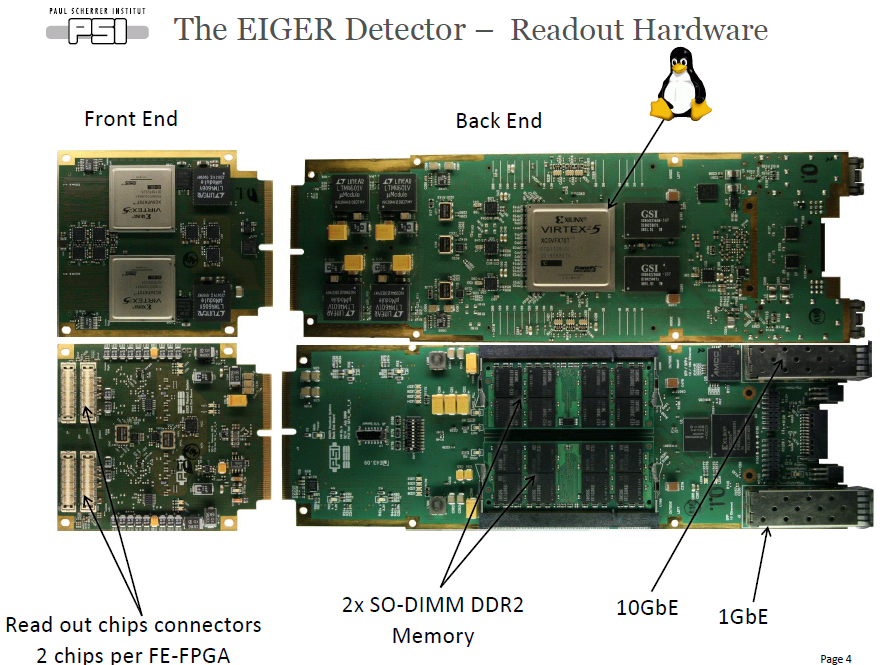
\includegraphics[width=1\textwidth]{Boards}
\end{center}
\caption{Picture with most relevant components of the EIGER readout system. The readout system starts with the Front End Boards (FEB) which performs data descrambling (also converts the packets from 12 $\to$ 16 bits) and rate correction. The BackEndBoard (BEB) has 2x2GB DDR2 memories and can perform data buffering (storing images on board) and data summation (16 bit $\to$ 32 bits). The controls to the detector are passed through the 1Gb, while in most installations, the data are sent out through the 10~GB ethernet connection.} 
\label{boards}
\end{figure}

\subsection{Mandatory setup - Hardware}
An EIGER single module (500~kpixels) needs:
\begin{itemize}
\item A chilled (water+alcohol) at 21~$^{\circ}$C for a single module (500k pixels), which needs to dissipate 85~W (every module, i.e. for two half boards). For the 9M, 1.5M, a special cooling liquid is required: 2/3 deionized water and 1/3 ESA Type 48. This is important as the high temperature generated by the boards accelerate the corrosion due to Cu/Al reaction and the blockage of the small channels where the liquid flows, in particular near the face of the detector and if it is a parallel flow and not a single loop. The 9M and 1.5M run at 19~$^{\circ}$C.  
\item A power supply (12~V, 8~A). For the 9~M, a special cpu is give to remotely switch on and off the detector: see section~\ref{bchip100}. 
\item 2$\times$1~Gb/s Ethernet connectors to control the detector and, optionally, receive data at low rate. A DHCP server that gives IPs to the 1~Gb/s connectors of the detector is needed. Note that flow control has to be enabled on the switch you are using, if you plan to read the data out from there. If not, you need to implement delays in the sending out of the data.
\item 2$\times$10~Gb/s transceivers to optionally, receive data at high rate. The 10Gb/s transceiver need to match the wavelength (long/short range) of the fibers chosen by the beamline infrastructure.
\end{itemize}
The equipment scales linearly with the number of modules.
Figure~\ref{fig:1} shows the relationship between the \textbf{Client} (which sits on a beamline control PC), the \textbf{Receiver} (which can run in multiple instances on one or more PCs which receive data from the detector. The receiver(s) does not necessary have to be running on the same PC as the client.) The username under which the receiver runs is the owner of the data files, if using our implementation. It is important that the receiver is closely connected to the detector (they have to be on the same network). Note that if you implement the 1Gb/s readout only: client, receiver and detector have to be all three in the same network. If you implement the 10Gb/s readout, then client, the 1~GbE of the detector and the receiver have to stay on the 1GbE. But the receiver data receiving device and the 10GbE detector can be on their private network, minimizing the missing packets.  

\begin{figure}[t]
\begin{center}
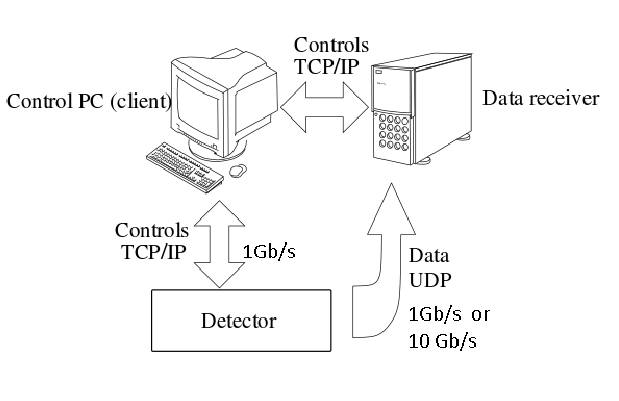
\includegraphics[width=.8\textwidth]{Client2}
\end{center}
\caption{Communications protocol between the Client PC, the receiver PC and the detector.}
\label{fig:1}
\end{figure}

The Client talks to control over 1~Gb Ethernet connection using TCP/IP to the detector and to the receiver. The detector sends data in UDP packets to the receiver. This data sending can be done over 1~Gb/s or 10~Gb/s. 
 
\begin{itemize}
\item \textbf{Switch on the detector only after having started the chiller: the 500k single module and the 1.5M at cSAXS/OMNY have a hardware temperature sensor, which will power off the boards if the temperature is too high. Note that the detector will be power on again as soon as the temperature has been lowered. The 9M will not boot up without the correct waterflow and temperature has it has an integrated flowmeter.} 
\item \textbf{Switch on the detector only after having connected all the cables and network. EIGER is unable to get IP address after it has been switched on without a proper network set up. In that case switch off and on the detector again.}
\end{itemize}

\subsubsection{9M power supply interface: bchip100}\label{bchip100}
So the bchip100, which is a blackfin cpu, is located on the top side of the 9M and needs to be connected over 1Gb, to the same or a different network as the detector 1~GbE. 
 \begin{verbatim}
telnet bchip100
cd 9m/
\end{verbatim}
The directory contains some executables that are needed to make your detector to work:
 \begin{verbatim}
./on #to switch modules on
./off #to switch modules off
./state #tells you if is ON or OFF
cat /var/log/pcu.log #displays the log if there are problem
./waterflow #returns the current waterflow returned by the flowmeter
./temp #returns the water temperature returned by the flowmeter
 \end{verbatim}
A watchdog is running on bchip100 to check for the flow and temperature. If outside of parameters ( flow$<$ 80 dl/min, temperature $\neq$21$\pm$2), the detector will be switched off. 
Here is an explanation of the LED color scheme of the bchip100: 
\begin{itemize}
\item NO LED  Main Power off or Blackfin not ready, yet.
\item RED     Too high temperature or too less water flow
        Detector is shut down and locked.
        Detector will be unlocked (YELLOW) automatically when conditions are good again.
\item YELLOW  Detector is off and unlocked. Ready to be turned on.
\item GREEN   Detector is on
\end{itemize}
You can also Check temperatures and water flow in a browser (from the same subnet where the 9M is: http://bchip100/status.cgi

\subsection{Mandatory setup - Receiver}

The receiver is a process run on a PC closely connected to the detector. Open one receiver for every half module board (remember, a module has two receivers!!!) . Go to {\tt{slsDetectorsPackage/build/bin/}}, \textbf{slsReceiver} should be started on the machine expected to receive the data from the detector.

\begin{itemize}
\item {\tt{./slsReceiver --rx\_tcpport xxxx}} 
\item {\tt{./slsReceiver --rx\_tcpport yyyy}}
\end{itemize}
where xxxx, yyyy are the tcp port numbers. Use 1955 and 1956 for example. The receiver for the bottom is open without arguments but still in the configuration file one needs to write {\tt{n:flippeddatax 1}}, where {\tt{2n+1}} indicated the half module number, 1 if it is a module.
\\ Open as many receiver as half module boards. A single module has two half module boards.

From the software version 3.0.1, one can decide weather start a zmq callback from the receiver to the client (for example to visualize data in the slsDetectorGui or another gui). If the zmq steam is not required (cased of the command line for example, one can switch off the streaming with {\tt{./sls\_detector\_put rx\_datastream 0}}, enable it with {\tt{./sls\_detector\_put rx\_datastream 1}}. In the case of initializing the stream to use the slsDetectorGui, nothing needs to be taken care of by the user. If instead you want to stream the streaming on different channels, the zmq port of the client can be set stealing from the slsDetectorGui stream having {\tt{./sls\_detector\_put zmqport 300y}}. Note that if this is done globally (not for every half module n independently, then the client automatically takes into account that for every half module, there are 2 zmq stream. The receiver stream {\tt{./sls\_detector\_put rx\_zmqport 300y}} has to match such that the GUI can work. 
If one desires to set the zmqport manually, he offset has to be taken into account: {\tt{./sls\_detector\_put 0:rx\_zmqport 300y}}, {\tt{./sls\_detector\_put 1:rx\_zmqport 300y+2}} and so on..


{\tt{slsMultiReceiver}} uses two or more receivers in one single terminal: {\tt{./slsMultiReceiver startTCPPort numReceivers withCallback}}, where startTCPPort assumes the other ports are consecutively increased.

The command {\tt{r\_framesperfile}} sets the number of frames written in the same file. By default now it is 10000. It can be changes. It needs to be lowered particularly if one wants to parallelize the following conversion of the files. 


\subsection{Mandatory setup - Client}

The command line interface consists in these main functions:
\begin{description}
\item[sls\_detector\_acquire] to acquire data from the detector
\item[sls\_detector\_put] to set detector parameters
\item[sls\_detector\_get] to retrieve detector parameters
\end{description}

First, your detector should always be configured for each PC that you might want to use for controlling the detector. All the examples given here show the command {\tt{0-}}, which could be omitted for the EIGER system $0$. In the case more EIGER systems are controlled at once, the call of {\tt{1-}},.. becomes compulsory. 

To make sure the shared memory is cleaned, before starting, one should do:  
\begin{verbatim}
sls_detector_get 0-free
\end{verbatim}
To do that:
\begin{verbatim}
sls_detector_put 0-config mydetector.config
\end{verbatim}

In the config file, if client, receiver and detector are using \textbf{1GbE} the following lines are mandatory (see slsDetectorsPackage/examples/eiger\_1Gb.config):
\begin{verbatim}
detsizechan 1024 512 #detector geometry, long side of the module first
hostname beb059+beb058+ #1Gb detector hostname for controls
0:rx_tcpport 1991 #tcpport for the first halfmodule                 
0:rx_udpport 50011 #udp port first quadrant, first halfmodule         
0:rx_udpport2 50012 #udp port second quadrant, first halfmodule       
1:rx_tcpport 1992 #tcpport for the second halfmodule               
1:rx_udpport 50013 #udp port first quadrant, second halfmodule       
1:rx_udpport2 50014 #udp port second quadrant, second halfmodule      
rx_hostname x12sa-vcons #1Gb receiver pc hostname
outdir /sls/X12SA/data/x12saop/Data10/Eiger0.5M
threaded 1
\end{verbatim}

In the config file, if client, receiver and detector commands are on 1Gb, but detector data to receiver are sent using \textbf{10GbE} the following lines are mandatory (see slsDetectorsPackage/examples/eiger\_10Gb.config):
\begin{verbatim}
detsizechan 1024 512 #detector geometry, long side of the module first
hostname beb059+beb058+ #1Gb detector hostname for controls
0:rx_tcpport 1991 #tcpport for the first halfmodule                 
0:rx_udpport 50011 #udp port first quadrant, first halfmodule       
0:rx_udpport2 50012 #udp port second quadrant, first halfmodule       
0:rx_udpip 10.0.30.210 #udp IP of the receiver over 10Gb              
0:detectorip 10.0.30.100  #first half module 10 Gb IP 
1:rx_tcpport 1992 #tcpport for the second halfmodule                  
1:rx_udpport 50013 #udp port first quadrant, second halfmodule     
1:rx_udpport2 50014 #udp port second quadrant, second halfmodule  
1:rx_udpip 10.0.40.210  #udp IP of the receiver over 10Gb, 
                        can be the same or different from 0:rx_udpip                                   
1:detectorip 10.0.40.101 #second half module 10 Gb IP 
rx_hostname x12sa-vcons #1Gb receiver pc hostname
outdir /sls/X12SA/data/x12saop/Data10/Eiger0.5M
threaded 1
\end{verbatim}

The geometry on af an EIGER module, showing the quadrants corresponding to the udp ports and the 2 receivers is shown in figure~\ref{fig:eigerports}.
\begin{figure}[t]
\begin{center}
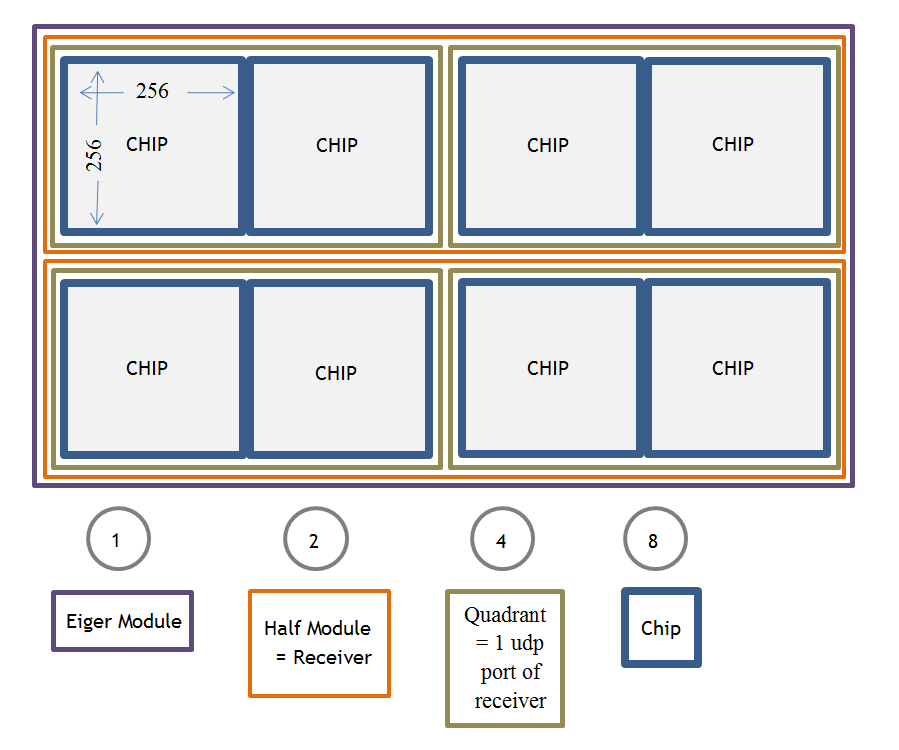
\includegraphics[width=0.9\textwidth]{Eiger-Chips}
\end{center}
\caption{Geometry of UDP ports and receivers in a singel module.}
\label{fig:eigerports}
\end{figure}

In the case you are developing your own receiver, then you need to remove the 1Gb receiver hostname {\tt{rx\_hostname}} and substitute it with the mac address of the device:
\begin{verbatim}
configuremac 0
rx_udpmac xx:xx:...
\end{verbatim}

One can configure all the detector settings in a parameter file {\tt{setup.det}}, which is loaded by doing:
\begin{verbatim}
sls_detector_put 0-parameters setup.det
\end{verbatim}

In the case of \E, the proper bias voltage of the sensor has to be setup, i.e. the {\tt{setup.det}} file needs to contain the line {\tt{vhighvoltage 150}}. Other detector functionality, which are rarely changed can be setup here. 
Other important settings that are configured in the {\tt{setup.det}} file are:
\begin{itemize}
\item {\tt{tengiga 0/1}}, which sets whether the detector is enabled to send data through the 1~or the 10~Gb Ethernet.
\item {\tt{flags parallel/nonparallel}}, which sets whether the detector is set in parallel acquisition and readout or in sequential mode. This changes the readout time of the chip and affects the frame rate capability (faster is {\tt{parallel}}, with higher noise but needed when the frame rate is $>2$~kHz. 
\item {\tt{dr 32/16/8/4}} sets the detector in autosumming mode (32 bit counter or not autosumming, 12 bit out of the chip). This is strictly connected to what is required for the readout clock of chip. See next point.
\item {\tt{clkdivider 0/1/2}}. Changes the readout clock: 200, 100, 50~MHz (also referred to as full, half, quarter speed). Note that autosumming mode ({\tt{dr 32}} only works at {clkdivider 2}=quarter speed). By selecting Refer to readout timing specifications in~section\ref{timing} for how to set the detector. 
\item {\tt{flags continuous/storeinram}}. Allows to take frame continuously or storing them on memory. Users should use the {\tt{continuous}} flags. Enabling the {\tt{stroreinram}} flag makes the data to be sent out all at the end of the acquisition. Refer to readout timing specifications in section~\ref{timing} for how to set the detector. Examples will be given in section~\ref{}.
\end{itemize}

One should notice that, by default, by choosing the option {\tt{dr 32}}, then the software automatically sets the detector to  {\tt{clkdivider 2}}. By choosing the option {\tt{dr 16}}, the software automatically sets the detector to  {\tt{clkdivider 1}}. One needs to choose {\tt{clkdivider 0}} after setting the {\tt{dr 16}} option to have the fastest frame rate. 
We would recommend expert users (beamline people) to write their parameters file for the users. 

\section{API versioning} \label{api}
The eigerDetectorServer running on the boards has a versioning API scheme that will make it crash if used with a wrong firmware.
You can also check your versioning by hand with the code:
\begin{verbatim}
 sls_detector_get softwareversion
\end{verbatim}
gets the server (slsDetectorSoftware) version (answer is something like: {\tt{softwareversion 111920160722}}.
 \begin{verbatim}
sls_detector_get thisversion 
\end{verbatim}
returns the client version. The answer can be {\tt{thisversion 111220160718}}.
\begin{verbatim}
/sls_detector_get detectorversion
\end{verbatim}
returns the firmware version . The answer can be {\tt{detectorversion 11}}.
Killing and starting the server on the boards allows you to check the firmware version you have and also if your board is a top/bottom/master/slave.

\section{Setting up the threshold}
\begin{verbatim}
sls_detector_put 0-trimen N xxxx yyyy zzzz
sls_detector_put 0-settings standard 
sls_detector_put 0-threshold energy_in_eV standard
\end{verbatim}
The first line requires to specify how many ({\tt{N}}) and at which energies in eV {\{tt{xxxx}}, {\tt{yyyy}}, {\tt{zzzz}} and so on) trimmed files were generated (to allow for an interpolation). This line should normally be included into the {\tt{mydetector.config}} file and should be set for you by one of the detector group.
NORMALLY, in this new calibration scheme, only {\tt{settings standard}} will be provided to you, unless specific cases to be discussed.
The threshold at 6000 eV , for example would be set as:{\tt{sls\_detector\_put 0-threshold 6000 standard}}.

For \E, at the moment normally only {\tt{standard}} settings are possible.
 {\tt{lowgain}}, {\tt{verylowgain}}, {\tt{veryhighgain}} and {\tt{highgain}} are theoretically possible, but we never calibrate like this. They could be implemented later if needed. 

Notice that setting the threshold actually loads the trimbit files (and interpolate them between the closest calibration energies) so it is time consuming. 
The threshold is expressed in (eV) as the proper threshold setting, i.e. normally is set to 50\% of the beam energy.  

We have added a special command, {\tt{thresholdnotb}}, which allows to scan the threshold energy without reloading the trimbits at every stage. One can either keep the trimbits at a specific value (es.32 if the range of energies to scan is large) or use the trimbits from a specific energy (like a central energy).
\begin{verbatim}
sls_detector_put 0-thresholdnotb energy_in_eV
\end{verbatim}
See section~\ref{sec:fastthresholdscan}.

\section{Standard acquisition}

After you setup the setting and the threshold, you need to specify the exposure time, the number of real time frames and eventually how many real time frames should be acquired:
\begin{verbatim}
sls_detector_put 0-exptime 1[time_is_s]
sls_detector_put 0-frames 10
sls_detector_put 0-period 0[time_is_s]
\end{verbatim}
In this acquisition 10 consecutive 1~s frames will be acquired. Note that {\tt{period}} defines the sum of the acquisition time and the desired dead time before the next frame. If {\tt{period}} is set to 0, then the next frame will start as soon as the detector is ready to take another acquisition. \\

%\underline{At cSAXS, the {\tt{settingsdir}} and {\tt{caldir}} are in}\\\underline{/sls/X12SA/data/x12saop/EigerPackage/calibrations/}\\ 

You need to setup where the files will be written to
\begin{verbatim}
sls_detector_put 0-outdir /scratch
sls_detector_put 0-fname run
sls_detector_put 0-index 0
\end{verbatim}
this way your files will all be named /scratch/run\_dj\_i.raw where $j$ is relative to each specific half module, $i$ in the {\tt{index}} starts from 0 when starting the detector the first time and is automatically incremented. The next acquisition {\tt{index}} will be 1. One can reset the  {\tt{index}} to what wished.

To acquire simply type:
\begin{verbatim}
sls_detector_acquire 0-
\end{verbatim}
Note that acquiring is blocking.
You can poll the status of the detector with:
\begin{verbatim}
sls_detector_get status
\end{verbatim}
If the detector is still acquiring, the answer will return {\tt{running}}. If the detector has finished and ready for the next acquisition, then it will return {\tt{idle}}.
You can also ask for the status of the receiver, to know when it has returned and finished getting the data with:
\begin{verbatim}
sls_detector_get receiver
\end{verbatim}

There is a more complex way of performing an acquisition, that is useful for debugging and in case one wants a non blocking behavior: 

You can then reset to zero the number of frames caught, then  start the receiver and the detector:
\begin{enumerate}
\item {\tt{sls\_detector\_put 0-resetframescaught 0}} 
\item {\tt{sls\_detector\_put 0-receiver start}} 
\item {\tt{sls\_detector\_put 0-status start}} 
\end{enumerate}

You can poll the detector status using:
\begin{verbatim}
sls_detector_get 0-status 
\end{verbatim}
When the detector is {\tt{idle}}, then the acquisition is done but the receiver could still be receiving data. If you want, you can check if the receiver is finished receiving as many frames as you were expecting (this is optional but required for many many frames acquisition or when using some delays to send data at very high frame rate.
\begin{enumerate}
\setcounter{enumi}{3}
\item {\tt{sls\_detector\_get framescaught}} 
\end{enumerate}
Then you can stop the receiver as well now:
\begin{enumerate}
\setcounter{enumi}{4}
\item {\tt{sls\_detector\_put 0-receiver stop}} 
\end{enumerate}

The detector will not accept other commands while acquiring. If an acquisition wishes to be properly aborted, then:
\begin{itemize}
\item {\tt{sls\_detector\_put 0-status stop}} 
\end{itemize}
this same command can be used after a non proper abortion of the acquisition to reset to normal status the detector.

\section{Gap pixels inside a module}
A module is composed of 2$\times$4 chips. Each chip is of dimension 256$\times$256 pixels. There is no dead area in a module, as a single sensor covers the 8 chips. The physical pixels at the border of the chips in the sensor are double in size, to allow not to loose photons in the gaps between the chip alignment. They count double what the other normal pixels would count. In the corner between chips, the pixels are 4-times the normal size. See figure~\ref{fgappix} to check the geometry.

\begin{figure}[t]
\begin{center}
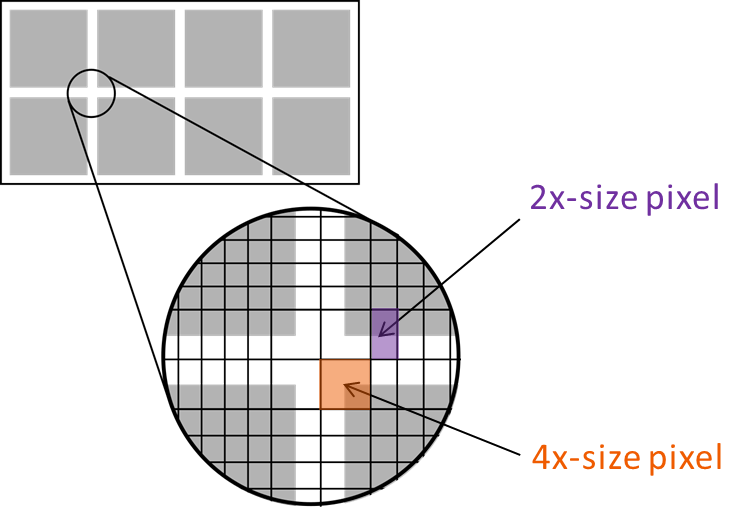
\includegraphics[width=0.9\textwidth]{GapPixels}
\end{center}
\caption{Geometry of gap pixels between a module.}
\label{fgappix}
\end{figure}

It is possible to interpolated the value on the larger pixels by splitting the events (or properly interpolating) introducing a virtual pixel for every double pixel, or 3 virtual pixels for every corner. In this way the counts of a single large pixel can be shared among the correct amount of pixels of the normal dimension.     

The gap pixels can be added for the slsDetectorGui, from the datacall back or stealing the zmq port from the GUI (see later). The detector size can be added in the configuration file as first thing. 

Putting the long side of the module first always as a convection for the code, WITHOUT GAP PIXELS an EIGER module is:
\begin{verbatim}
detsizechan 1024 512 
\end{verbatim}
and the client needs to be set {\tt{sls\_detector\_put  gappixels 0}}, which is the default behavior.\\
If you want to have GAP PIXELS included: 
\begin{verbatim}
detsizechan 1030 514 
\end{verbatim}
and the client needs to be set {\tt{sls\_detector\_put  gappixels 1}}.

The size of the gap pixels between modules to insert is 
\begin{verbatim}
   GapPixelsBetweenModules_x = 8
   GapPixelsBetweenModules_y = 36
\end{verbatim}
where the {\tt{GapPixelsBetweenModules\_x}} are the one on the short side of the module, while {\tt{GapPixelsBetweenModules\_y}} are the ones on the long side of the module (where the wirebonds take physical space).
  \section{QUAD special geometry}
Starting from release 4.1.0, we support a special geometry with 2x2 pixels. This is for a Quad, where a single half module reads out 4 chips but in a quad shape. For now this hardware is only available as a PEEM detector at SIM. 
The {\tt{detsizechan 1024 512}} needs to remain set like this for a half module. However, thanks to the command: 
 \begin{verbatim}
./sls_detector_put quad 1
\end{verbatim}

a 512x512 geomtry will be read out if {\tt{gappixels 0}} and 514x514 will be readout if {\tt{gappixels 1}}. Note that as above, {\tt{gappixels 1}} is not supported for {\tt{dr 4}}.   
If  {\tt{gappixels 0}}, in the master.raw file you will read: 
\begin{verbatim}
row                        : 512 pixels
col                        : 256 pixels
\end{verbatim}
else if {\tt{gappixels 1}}, in the master.raw file you will read: 
\begin{verbatim}
row                        : 514 pixels
col                        : 257 pixels
\end{verbatim}

\section{Readout timing- maximum frame rate}\label{timing}
IMPORTANT: to have faster readout and smaller dead time, one can configure {\tt{clkdivider}}, i.e. the speed at which the data are read, i.e. 200/100/50~MHz for {\tt{clkdivider 0/1/2}} and the dead time between frames through {\tt{flags parallel}}, i.e. acquire and read at the same time or acquire and then read out.
The configuration of this timing variables allows to achieve different frame rates. NOTE THAT IN EIGER, WHATEVER YOU DO, THE FRAME RATE LIMITATIONS COME FROM THE NETWORK BOTTLENECK AS THE HARDWARE GOES FASTER THAN THE DATA OUT.

In the case of REAL CONTINUOUS readout, i.e. continuous acquire and readout from the boards (independent on how the chip is set), the continuous frame rates are listed in table~\ref{tcont}. The time to send out the frame out of the board 
\begin{table} 
\begin{tabular}{|c|c|c|c|c|}
\hline
\tiny{GbE} & \tiny{dynamic range} & \tiny{continuos maximum frame rate(Hz)} & \tiny{minimum period ($\mu$s)}& \tiny{time to send out data ($\mu$s)}\\
\hline
1 & 16 &  \textbf{256} & 3901 & \\ 
\hline 
1 &  32 &  \textbf{128} & 7820 & \\
\hline 
10 & 4 & \textbf{10240} & 98 & 100\\
\hline 
10 & 8 & \textbf{5120} & 196 & 200\\
\hline
10 & 16 & \textbf{2560} & 391 & 400\\  
\hline 
10 & 32 & \textbf{1280} & 782 & 800\\  
\hline 
\end{tabular}
\caption{Frame rate limits for the CONTINUOS streaming out of images, i.e. the data rate out is just below 1Gb/s or 10Gb/s. 1280~Hz for 32-bit, 10GbE is obtained from the 10GbE limitation. The maximum achievable frame rate is 977~Hz.} 
\label{tcont}\end{table}
 Note that in the {\tt{continuous}} flag mode, some buffering is still done on the memories, so a higher frame rate than the proper real continuous one can be achieved. Still, this extra buffering is possible till the memories are not saturated. The number of images that can be stored on the DDR2 on board memories are listed in table~\ref{timgs}.
\begin{table}
\begin{tabular}{|c|c|}
\hline
dynamic range & images\\
\hline
4 & 30000\\
\hline
8 & 15000\\
\hline
16 & 7600\\
\hline
\end{tabular}
\caption{Amount of images that can be stored on board. As while we store them, we start to send them out, the effective number of images could be larger than this, but it will depend on the network setup (how fats you stream out images).}
\label{timgs}
\end{table}

The maximum frame rate achievable with 10~GbE, {\tt{dr 16}}, {\tt{flags continuous}}, {\tt{flags parallel}},{\tt{clkdivider 0}}, \textbf{6.1~kHz}. This is currently limited by the connection between the Front End Board and the Backend board. We expect the 32 bit mode limit, internally, to be \textbf{2~kHz} ({\tt{clkdivider 2}}).
 In dynamic range {\tt{dr 8}} the frame rate is \textbf{11~kHz} and for{\tt{dr 4}} is \textbf{22~kHz}. For 4 and 8 bit mode the frame rate are directly limited by the speed of the detector chip and not by the readout boards.    

\subsection{Minimum time between frames and Maximum frame rate}

We need to leave enough time between an exposure and the following. This time is a combination of the time required by the chip, by the readout boards and eventually extra time to reduce some appearance of cross talk noise between the digital and analog parts of the chip. 
\textbf{It is essential to set the {\tt{period}} of the detector, defined as the {\tt{exptime}} plus an extra time, that needs to be at least the chip/board readout time. If this is set wrong (it is $<$ {\tt{exptime}} plus chip/board readout time), then the detector takes the minimum time it can, but you are in a not controlled frame rate situation.} 

The expected time difference between frames given by the pure chip readout time is in Table~\ref{tchipro}.    
\begin{tiny}
\begin{table}
\begin{flushleft}
\begin{tabular}{|c|c|c|c|}
\hline
\tiny{dr} & \tiny{clkdivider} & \tiny{expected chip readout t($\mu$s)} & \tiny{measured chip readout t($\mu$s)}\\
\hline
4 & 0 & 41 & 40\\
4 & 1 & 82 & 84\\
4 & 2 & 123 & 172\\
\hline
\hline
8 & 0 & 82 & 82\\
8 & 1 & 164 & 167\\
8 & 2 & 328 & 336\\
\hline
\hline
12 & 0 & 123 &122\\
12 & 1 & 246 & 251\\
12 & 2 & 491 & 500\\
\hline
\end{tabular}
\caption{Readout time required from the chip to readout the pixels. The numbers are obtained using equation~\ref{dtnonparallel}.}
\label{tchipro}
\end{flushleft}
\end{table}
\end{tiny}

The {\tt{period}} is s is defined as:
\begin{equation} \label{period}
\textrm{period}  = \textrm{exptime} + \textrm{minimum time between frames}
\end{equation}
where the 'minimum time between frames' and the minimum period will be discussed in Table~\ref{tframes}.
\begin{tiny}
\begin{table}
\begin{flushleft}
\begin{tabular}{|c|c|c|c|c|c|c|c|}
\hline
\tiny{dr} & \tiny{clkdivider} & \tiny{flags} & \tiny{$\Delta$t frames($\mu$s) } &  \tiny{max FR (kHz)} & \tiny{min period ($\mu$s)} & \tiny{meas. period ($\mu$s)} & \tiny{max imgs (nominal/our network)}\\
\hline
4 & 0 & \tiny {parallel} & 3.4 & 22  & 44 & 44.01 & 30k/50k\\
\hline
\hline
8 & 0 & \tiny {parallel} & 3.4 & 11.1 & 89 & 89.01 & 15k/24k\\
\hline
16 & 0 & \tiny {parallel} & 3.4 & 6.1 & (126+38)* =164 & 164.02 & 8k/12k\\
\hline
16 & 0 & \tiny {nonparallel} &  127 & 5.6 & (126+52)*= 179 & 179.01& 8k/23k\\
\hline
16 & 1 & \tiny {parallel} &  6.1 & 3.9 &  257 & 257.01 & 8k/28k\\
\hline
16 & 1 & \tiny {nonparallel} & 255 & 3.3 &  303 & 303.01 & infinite\\
\hline
\end{tabular}
\caption{Readout settings. The {\tiny{min exptime}} possible is 5$-$10~$\mu$s. This is due to the time to pass the pixel enable signal in the whole chip. The time between frames ($\Delta$t) has been measured with the oscilloscope and the maximum frames rate (max FR) has been tested with an external gating from a pulse generator at known frequency. The minimum period is obtained as 1/$\textrm{max frame rate}$.}
\label{tframes}
\end{flushleft}
\end{table}
\end{tiny}

\textbf{From software version 4.0.0, there is a very useful function {\tt{sls\_detector\_get measuredperiod}} which return the measured period AFTER the acquisition. This is important to check that the settings to obtain the targeted frame rate was correct.} 

\textbf{If you run too fast, the detector could become noisier (see problem shooting), it is important to match the detector settings to your frame rate. This can be done having more parameters files and load the one suitable with your experiment.} We experienced that with low energy settings could not reach 6~kHz and no noise.
In 16 bit mode, it could make sense, in case of noise and low threshold to either reduce the frame rate:
\begin{equation} 
\textrm{new period}  = \textrm{exptime} + \textrm{minimum time between frames} + (\textrm{10$-$20 }\mu \textrm{s})
\end{equation}
to let the signal settle  or,  if the frame rate is important, leave the {\tt{period}} at the same value but reduce the {\tt{exptime}}:
\begin{equation} 
\textrm{new exptime}  = \textrm{old exptime} - (\textrm{10$-$20 }\mu \textrm{s})
\end{equation}

In general, choose the maximum frame rate you want to aim, not exceeding what you aim for not to increase the noise. In 4 and 8 bit modes it makes no sense to run nonparallel as the exposure time is too small compared to the readout time. 

Here below are the final tables for settting the detcetor correctly:

\begin{itemize}
\item CONTINUOUS redout (imagesnot stored on board memories,  frames can be achieved. {\tt{flags parallel}}, {\tt{clkdivider 0}} are always set. In 32-bit no extra {\tt{subdeadtime}} is assumed. The difference between {\tt{exptime}} and {\tt{period}} has to be $\approx$5 $\mu$s:
\begin{center}
  \begin{tabular}{ |c| c| } 
    \hline
    max frame rate & settings\\
    \hline
    \textcolor{red}{189~Hz (977~Hz max)} &  \textcolor{red}{32-bit} \\
    & Nframes=infinite\\
    \hline
      \textcolor{red}{2.56 kHz} &  \textcolor{red}{16-bit}\\
     & Nframes=infinite\\
     \hline
      \textcolor{red}{5.1 kHz} &  \textcolor{red}{8-bit}\\
     & Nframes=infinite\\
     \hline
      \textcolor{red}{10.2 kHz} &  \textcolor{red}{4-bit}\\
     & Nframes=infinite\\
     \hline
  \end{tabular}
\end{center}
BE CAREFUL that if you have the transmission delays setup (see sec.~\ref{network}), this will slow down the sending of the data and you risk to fill up the memories of the boards on eiger (30000 images in 4 bit mode) and you will get corrupted data (parts of the memory on the boads will be overwritten).

\item BUFFERED readout (images stored on board memories, such that the maximum frame rate can be achieved for a limited amount of frames. {\tt{flags parallel}}, {\tt{clkdivider 0}} are always set. In 32-bit no extra {\tt{subdeadtime}} is assumed. The difference between {\tt{exptime}} and {\tt{period}} has to be $\approx$5 $\mu$s:
\begin{center}
  \begin{tabular}{ |c| c| } 
    \hline
    max frame rate & settings\\
    \hline
    \textcolor{red}{189~Hz (977~Hz)} &  \textcolor{red}{32-bit} \\
    & Nframes=infinite\\
    \hline
     \textcolor{red}{6.1 kHz} &  \textcolor{red}{16-bit}\\
    & Nframes=7600\\
    \hline
     \textcolor{red}{11.1 kHz} &  \textcolor{red}{8-bit}\\
    & Nframes=15000\\
    \hline
     \textcolor{red}{22 kHz} &  \textcolor{red}{4-bit}\\
    & Nframes=30000\\
    \hline
  \end{tabular}
\end{center}
\end{itemize}



\subsubsection{4 and 8 bit mode}
In {\tt{parallel}} mode, the minimum time between frames is due to the time required to latch the values of the counter with capacitors. These values are determined in firmware and they can be estimated as:

\begin{equation} \label{dtparallel}
\textrm{time between frames, parallel} = 4 \mu s \cdot (clkdivider+1)
\end{equation}

This time is independent on the {\tt{dr}}.

In {\tt{nonparallel}} mode, it is easily possible to calculate the required asic readout time. 
Indeed a block of (8*256) pixels are readout, the bits pixel are the {\tt{dr}} and the speed of readout is 5ns/bit *({\tt{clkdivider}}+1) : 

\begin{equation}\label{dtnonparallel}
\textrm{asics readout time} = 5ns/bit \cdot 2^{(clkdivider+1)} \cdot dr \cdot (8*256) + 4 \mu s \cdot (clkdivider+1)
\end{equation}

While we expose the next frame, we still need to readout the previous frame, so we need to guarantee that the period is large enough at least to readout the frame. So the maximum frame rate has to be $1/(\textrm{asic readout time})$. The minimum period has to be equal to the asic readout time. 

\subsubsection{16 bit mode}

A similar situation happens in 16 bit mode, where this is more complicated because of three things:
\begin{enumerate}
\item The chip actual {\tt{dr}} is 12 bit
\item The chip is readout as 12-bit/pixel, but the FEB inflates the pixel values to 16-bits when it passes to the BEB. This means that effectively the FEB to BEB connection limits the data throughput in the same way as if the {\tt{dr}} of the chip would really be 16 bits.
\item While in 4 and 8 bit mode it makes no sense to run in {\tt{nonparallel}} mode as the exptime/dead time ratio would be not advantageous, in 16 bit mode, one can choose how to run more freely.
\end{enumerate}

If we are in parallel mode, the dead time between frames, is also here described by equation~\ref{dtparallel}. If we are in {\tt{nonparallel}} mode, the dead time between frames is defined by \ref{dtnonparallel} ONLY for {\tt{clkdivider}} 1 and 2. So the maximum frame rate has to be $1/(\textrm{chip readout time})$ in this case. Only for {\tt{clkdivider}} 0 we hit some limitation in the bandwidth of The FEB $\to$ BEB connection. In this case, the maximum frame rate is lowered compared to what expected.

\subsubsection{32 bit mode}
The autosumming mode of Eiger is the intended for long exposure times (frame rate of order of 100Hz, PILATUS like). A single acquisition is broken down into many smaller 12-bit acquisitions, each of a {\tt{subexptime}} of 2.621440~ms by default. Normally, this is a good default value to sustain an intensity of $10^6$ photons/pixel/s with no saturation. To change the value of {\tt{subexptime}} see section~\ref{advanced}. 

The time between 12-bit subframes are listed in table~\ref{t32bitframe}.  
\begin{tiny}
\begin{table}
\begin{flushleft}
\begin{tabular}{|c|c|c|c|c|c|c|}
\hline
\tiny{dr} & \tiny{clkdivider} & \tiny{flags} & \tiny{subexptime (s)} & \tiny{t difference between subframes($\mu$s)} & \tiny{max internal subframe rate (kHz)} & \tiny{maximum frame rate (Hz)}\\
\hline
32 & 2 & parallel & 0.00262144 & 12 & 380 & 189\\
\hline
32 & 2 & parallel & 0.000490 & 12 & 2 & 997\\
\hline
\end{tabular}
\caption{Timing for the 32bit case. The maximum frame rate has been computed assuming 2 subframes of default {\tt{subexptime}} of 2.62144 ms, which is the default value. By setting up {\tt{subexptime}} to 490~$\mu$s one can achieve a maximum frame rate. Note that one has to leave 490$\mu$s extra between a frame and the following.}
\label{t32bitframe}
\end{flushleft}
\end{table}
\end{tiny}

\textbf{The exposure time brokend up rounding up to the full next complete subframe that can be started.}
The number of subframes composing a single 32bit acquisition can be calculated as:
\begin{equation}
\textrm{\# subframes}= (int) (\frac{\textrm{exptime (s)}}{\textrm{subexptime (s) + difference between frames (s)}}+0.5)
%\label{esubframes}
\end{equation}
This also means that {\tt{exptime}}$<${\tt{subexptime}} will be rounded to{\tt{subexptime}}. If you want shorter acquisitions, either reduce the {\tt{subexptime}} or switch two 16-bit mode (you can always sum offline if needed).   

From release 4.0.0, an extra {\tt{flag overflow/nooverflow}} is added, with {\tt{nooverflow}} default:
\begin{itemize}
\item {\tt{nooverflow}}: the internal 12-bit result is summed, even if there was saturation of the 12-bit counter (4095) in any of the subframes. Note that if there is saturation for every subframe, you might get as a result a value of the counter equal to (4095$\times$~number~of~subframes), which you need to correctly identify. On the other hand if the saturation occurred only one time, you will get something "close'' to the real number.
\item {\tt{overflow}}: In this case, even if a pixel saturate only 1 time in a subframe, you will be returned as a value of the counter for that pixel: $2^{32}-1$, i.e. 4294967295.  
\end{itemize}

The UDP header will contain, after you receive the data, the effective number of subframe per image (see section~\ref{UDP}) as  "SubFrame Num or Exp Time", i.e. the number of subframes recorded  (32 bit eiger).
The effective time the detector has recorded data can be computed as:
\begin{equation}
\textrm{effective exptime}=(\textrm{subexptime})\cdot (\textrm{\# subframes})
%\label{esubframes}
\end{equation}

 From release 4.0.0, a configurable extra time difference between subframes can be introduced for the parallel mode, so that some noise appearing in detectors at low threshold can be removed. This is obtained through the {\tt{subdeadtime}}. You need to add values specific for your detector (ask the detector group). Typically, values between 15-40~$\mu$s should be used (for the 9M it is currently 200~$\mu$s due to a noisier module).



\section{External triggering options}\label{triggering}
The detector can be setup such to receive external triggers. Connect a LEMO signal to the TRIGGER IN connector in the Power Distribution Board (see Fig.). The logic 0 for the board is passed by low level 0$-$0.7~V, the logic 1 is passed to the board with a signal between 1.2$-$5~V. Eiger is 50~$\Omega$ terminated. By default the positive polarity is used (negative should not be passed to the board).

\begin{figure}[t]
\begin{center}
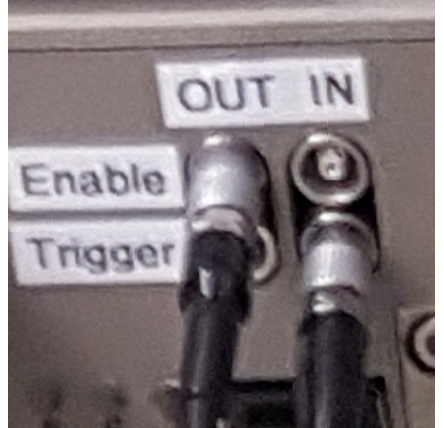
\includegraphics[width=.4\textwidth]{tiggerIN}
\end{center}
\caption{\textbf{Trigger INPUT} (looking at a single module from the back, top) is the \textbf{rightmost, down}.}
\label{triggerIN}
\end{figure}

\begin{verbatim}
sls_detector_put 0-timing [auto/trigger/burst_trigger/gating]
sls_detector_put 0-frames x
sls_detector_put 0-cycles y
sls_detector_acquire 0-
\end{verbatim}
No timeout is expected between the start of the acquisition and the arrival of the first trigger. 

Here are the implemented options so far:
\begin{itemize}
\item {\tt{auto}} is the software controlled acquisition (does not use triggers), where {\tt{exptime}} and {\tt{period}} have to be set. Set number of cycles (i.e. triggers) to 1 using {\tt{cycles}}. Set number of frames using {\tt{frames}}.
\item {\tt{trigger}} 1 frame taken for 1 trigger. Your {\tt{frames}} needs to be  1 always, {\tt{cycles}} can be changed and defines how many triggers are considered.  {\tt{exptime}} needs to be set. In the GUI this is called trigger exposure series.  
\item {\tt{burst\_trigger}} gets only 1 trigger, but allows to take many frames. With {\tt{frames}} one can change the number of frames. {\tt{cycles}} needs to be 1.  {\tt{exptime}} and {\tt{period}} have to be set. In the gui it is called trigger readout.
\item{\tt{gating}} allows to get a frame only when the trigger pulse is gating. Note that in this case the exp time and period only depend on the gating signal. {\tt{cycles}} allows to select how many gates to consider.  Set number of frames to 1 using {\tt{frames}}. IMPORTANT: Up to firmware 23, the last subframe is oblige to finish being taken, despite the gate signal going down. This will be configurable from later fw and software version. Also, in gating mode, due to timimg of the state machine, you need to leave 500~$\mu$s deadtime between the end on an acquisition and the next. This is as the state machine is unable to check for changes in the status in the first 500~$\mu$s. ATTENTION: if you are in 16 bit mode and you are applying online rate corrections, as now the exptime is generated by the trigger, you might not have correct rate corrections. If you know what the exposure time is in the gating signal, then you can set the {\tt{exptime}} once and the rate corrections will be correct. In 32 bit mode, it does not matter as the rate corrections depends on the {\tt{subexptime}} which is software set independently from the gate exptime.

When using 32-bit mode, by default the acquisition ends the last complete subframe that was started when still the acquisition time was valid. This has been chosen as many people wants to know the exact acquisition time for when the detector was taking data and also, if {\tt{ratecorr}} are active, the last subframe will be correctly corrected, while otherwise it will be corrected with a wrong subdeadtime. 
However, from 4.1.0, in gating mode, an option to immediately terminate the subframe when the gate signal goes down it is implemented to stop the acquisition at the same time.  This option is {\tt{./sls\_detector\_put interruptsubframe 1}} while the default option is {\tt{./sls\_detector\_put interruptsubframe 0}}.  

\end{itemize}

Hardware-wise, the ENABLE OUT signal outputs when the chips are really acquiring. This means that the single subframes will be output in 32 bit mode. The TRIGGER OUT outputs the sum-up-signal at the moment (which is useless). This will be changed in the future to output the envelop of the enable signal. 

We are planning to change some functionality, i.e. unify the {\tt{trigger}} and {\tt{burst\_trigger}} trigger modes and make both {\tt{frames}} and {\tt{cycles}} configurable at the same time.

There is the possibility to use {\tt{timing trigger/burst\_trigger}} and send software single commands to fake the trigger. This is done with:
\begin{verbatim}
sls_detector_put 0-timing [trigger/burst_trigger]
sls_detector_put 0-frames x
sls_detector_put 0-cycles y
sls_detector_status trigger
\end{verbatim}
 Note that this functionality is very (!) useful if you need to do something between and acquisition and the next. This can be used to do a fast threshold scan for example. See section~\ref{sec:fastthresholdscan}.


\section{Autosumming and rate corrections} \label{advanced}

In the case of autosumming mode, i.e, {\tt{dr 32}}, the acquisition time ({\tt{exptime}} is broken in as many subframes as they fit into the acquisition time minus all the subframes readout times. By default the {\tt{subexptime}} is set to 2.621440~ms. This implies that 12 bit counter of \E will saturate when the rate is above or equal to 1.57~MHz/pixel. The minimum value is of order of 10~ns (although as explained values smaller than 500~$\mu$s do not make sense). The maximum value is 5.2~s.

The subframe length can be changed by the user by doing: 
\begin{verbatim}
sls_detector_put 0-subexptime [time_in_s] 
\end{verbatim}

One needs to realize that the readout time, for each subframe is 10.5~$\mu$s if the detector is in parallel mode. 500~$\mu$s if the detector is in non parallel mode. Note that in {\tt{dr 32}}, as the single frame readout from the chip is 500~$\mu$s, no {\tt{subexptime}}$<$500~$\mu$s can be set in {\tt{parallel}} mode. To have smaller {\tt{subexptime}}, you need the {\tt{nonparallel}} mode, although this will have a larger deadtime than the acquisition time.\\

Rate corrections are possible online (and the came procedure can be used offline) by creating a look-up table between the theoretically incident counter value $c_i$ and the detected counter value $c_d$. 
In the EIGER on board server, this look-up table is generated assuming that the detected rate $n_d$ can be modeled as a function of the incident rate $n_i$ according to the paralyzable counter model:
\begin{equation}
n_d= n_i \cdot exp(-n_i \cdot \tau),
\label{rate}
\end{equation}
where $\tau$ represents an effective parameter for the dead time and the loss in efficiency. The look-up table is necessary as we are interested to obtain $c_i(c_d)$ and equation~\ref{rate} is not invertible. One needs to notice that the paralyzable counter model to create a look-up tables applies only if photons arrive with a continuous pattern (like at the SLS). If photons are structured in fewer but intenser bunches, deviations may arise. This is the case for some operation modes at the ESRF. For those cases we are studying how to correct, probably from a simulated correction tables if an analytical curve cannot be found.  
\textbf{In the new calibration scheme, $\tau$ is given as a function of the energy. It is loaded from the trimbit files and interpolation between two trimbit files are performed.} One needs to make sure the appropriate $\tau$ value is written in the trimbit files, then need to load the appropriate {\tt{settings}} and {\tt{vthreshold}} before.

Online rate corrections can be activated for {\tt{dr=32}}. They are particularly useful in the autosumming mode as  every single subframe is corrected before summing it. To correct for rate, the subframe duration has to be known to the correction algorithm. Rate corrections for {\tt{dr=16}} will be activated as well in the next firmware release.     
To activate the rate corrections, one should do:\\
\begin{verbatim}
sls_detector_put 0-ratecorr [tauval_in_ns]
\end{verbatim}
To deactivate:
\begin{verbatim}
sls_detector_put 0-ratecorr 0
\end{verbatim}

 Now to activate the rate corrections with the value written in the trimbit file or interpolated from there, once would do: 
\begin{verbatim}
sls_detector_put 0-ratecorr -1
\end{verbatim}

Every time either the rate corrections are activated, $\tau$ is changed or the subframe length is changed, then a new correction table is evaluated. Note that computing the correction table is time consuming. 

Here in figure~\ref{rateplots} you can find typical values of $\tau$  and typical values of the rates for which we have small non linerities (10\% non linearity) as a function of the beam energy.
\begin{figure}[t]
\begin{center}
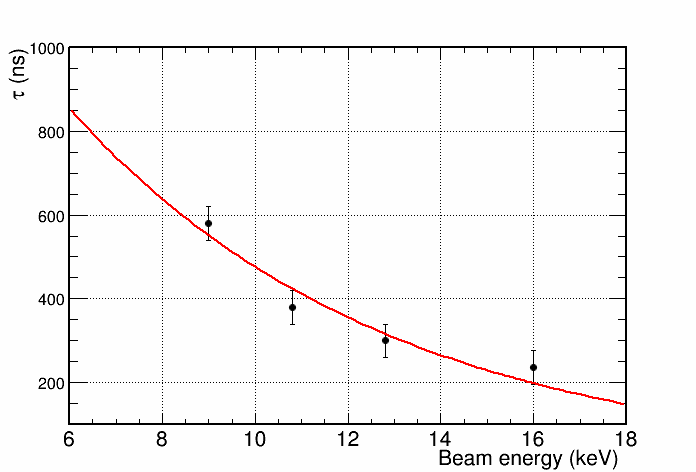
\includegraphics[width=.7\textwidth]{tauvsE}
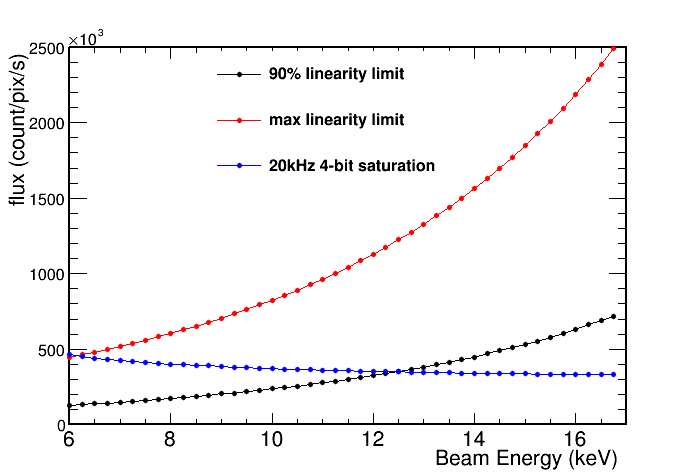
\includegraphics[width=.7\textwidth]{Ratecapabilityflux}
\end{center}
\caption{Typical values of the dead time for the detector and safe fluxes as a function of the beam energy}.
\label{rateplots}
\end{figure}




\section{Dependent parameters and limits}
Here is a list of dependent parameters:
\begin{enumerate}
\item \textbf{dr} changes \textbf{clkdivider}: \textbf{dr} 16 $\to$  \textbf{clkdivider} 1. You can change it to (0, 1, 2); the frame rate changes accordingly to table~\ref{tframes}. Setting the \textbf{dr} to 32 changes \textbf{clkdivider} to 2. Only way  \textbf{dr} 32 can work. 
\end{enumerate}

Here is a list of "ignored'' parameters, meaning that if the parameters are not what the detector expects, it will ignore them, but there is no guarantee that you get what you think you are asking: 
\begin{enumerate}
\item \textbf{period}. Assuming that you set the correct \textbf{exptime} according to the table~\ref{tframes}, the \textbf{period} to be used by the detector has to be $>=$ \textbf{exptime}+readout time (table~\ref{tframes}). Otherwise the detector will take data at the minimum possible period, which is \textbf{exptime}+readout times. \textbf{period} is not changed by the detector after the acquisition. 
\end{enumerate}

Here is a list of limits that should be checked:
\begin{enumerate}
\item 
If \textbf{dr} is 32 and \textbf{clkdivider} is not 2, whatever the detector gets out is wrong (the boards cannot properly keep up) 
\item If the variable \textbf{frames} is greater than what the memory can store (table~\ref{timgs}) and the frame rate exceed the continuos streaming (table~\ref{tcont}), limits on the maximum number of images need to be implemented if the period is lower than the one listed in table~\ref{tcont}. Check table~\ref{tframes} to see the different cases.
\item Running at a speed that does not support the frame rate you are asking: see table~\ref{tframes} to check if the frame rate (\textbf{period}) you are asking is compatible with the \textbf{clkdivider} you are asking.
\item Running at a readout time that does not support the frame rate you are asking. Check table~\ref{tframes} to check if the frame rate (\textbf{period}) you are asking is compatible with the \textbf{flags} you are asking.
\item The minimum allowed value for \textbf{exptime} should be 10~$\mu$s. 
\item By default the {\textbf{subexptime}} is set to 2.621440~ms. Values smaller than 500~$\mu$s do not make sense. The maximum value is 5.2~s. This limits should be checked.
\end{enumerate}

Here is a list of parameters that should be reset:
\begin{enumerate}
\item  \textbf{resetframescaught} should be reset to zero after every acquisition taken with {\tt{receiver start}},{\tt{status start}},{\tt{receiver stop}}. If the acquisition is taken with {\tt{sls\_detector\_acquire}}, there is no need to reset this.
\item After changing the {\tt{timing}} mode of the detector, one should reset to '1' the unused value, in that specific timing mode, between \textbf{frames} and \textbf{cycles}. See section~\ref{triggering} for how to use the timing. At the present moment the detector will acquire more frames than planned if the variable not used between \textbf{frames} and \textbf{cycles} is not reset. In future releases, the unused variable will be ignored. Still resetting is a good practice.
      
\end{enumerate}

\section{1Gb/s, 10Gb/s links}
\subsection{Checking the 1Gb/s, 10Gb/s physical links}\label{led}
LEDs on the backpanel board at the back of each half module signal:
\begin{itemize}
\item  the 1Gb/s physical link is signaled by the most external LED (should be green). For top half modules is at the extreme left. For bottom half modules is at the extreme right.  
\item the 10Gb/s physical link is signaled by the second most external LED next to the 1Gb/s one (should be green). 
\end{itemize}

\begin{figure}[t]
\begin{center}
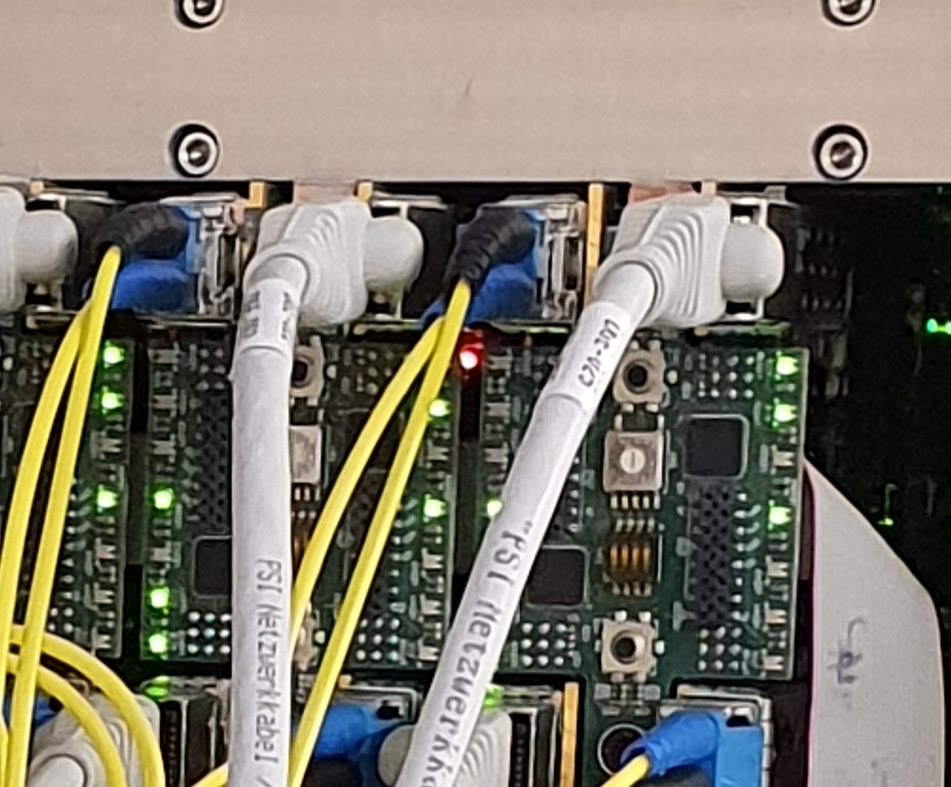
\includegraphics[width=.7\textwidth]{LEDSim}
\end{center}
\caption{1 and 10GB LEDs position.}
\label{fLEDs}
\end{figure}




\subsection{Delays in sending for 1Gb/s, 10Gb/s, 10Gb flow control, receiver fifo}\label{network}

Extremely advanced options allow to:
\begin{itemize}
\item Activate the flow control for 10~Gb/s~E (by default the 1~Gb/s~E is always active and cannot be switched off:
\begin{verbatim}
./sls_detector_put flowcontrol_10g 1
\end{verbatim}
\item  Delay the transmission of the left port. This delay option is useful in the case of many simultaneous receivers running, such that it reduces the throughput to the receivers all at the same time. To be used board by board (i.e {\tt{X:, Y:,etc..}} with different units:
\begin{verbatim}
./sls_detector_put X:txndelay_left xxxx 
\end{verbatim}
\item  Transmission delay of the right port, same as above. The value here should be different from the left port to spread the transmission even more 
\begin{verbatim}
./sls_detector_put X:txndelay_right yyyy
\end{verbatim}
As example:
\begin{verbatim}
for X in $(seq 0 4); do ./sls_detector_put $X:txndelay_left $((X*100000)); done
 \end{verbatim}
\begin{verbatim}
./sls_detector_put $X:txndelay_right $((X*100000)); X=$((X+1)); done
\end{verbatim}

\item Set transmission delay of the entire frame. This is required as you want to finish sending the first frame to all receivers before starting sending the second frame to the receivers with shorter delay time.  This value has to be greater than the maximum of the transmission delays of each port.      
\begin{verbatim}
./sls_detector_put txndelay_frame zzzz
\end{verbatim}
In the example before, it would be: {\tt{zzzz}}=4*100000+ 100000
To decide the size of the transmission delays, look at subsection~\ref{delays}. 

\item Readjust the size of the fifo of the receiver between listening and writing (useful when writing is limited)
\begin{verbatim}
./sls_detector_put rx_fifodepth xxxx
\end{verbatim}
 {\tt{xxxx}} is 100 images by default.
\item Deactivate a half module (for ROI or debugging). Note that the MASTER module SHOULD NOT be deactivated:
\begin{verbatim}
./sls_detector_put X:activate 0 
\end{verbatim}
where $X$ is the half module you want to deactivate.
The receiver at this point will return fake data (overflow) for this module. If you wish to eliminate the receiver overall for this module, then you need to run a configuration file where this module has been removed.
To activate back a module, do:
\begin{verbatim}
./sls_detector_put X:activate 1
\end{verbatim}

\end{itemize}

\section{Choose correct transmission delays}\label{delays}

Transmission delays should be chosen only to accomodate the writing speed of the disk. The 10Gb network should be optimised independently to allow no packet loss situation. This can be done by turning off the writing of the files and check only for missing frames. 

Table~\ref{tcont} gives the times that are needed to transfer 1 images out of the 10~Gb Ethernet connection. This reflects the CONTINUOS frame rate achieavable. The disk speed can be monitored with {\tt{dstat}}. One you have worked out this, you can calculated the {\tt{txndelay\_frame}} delay as:

\begin{equation}
 {\tt{txndelay\_frame}}=-tsending+dr \cdot \frac{4*256*256*N\_half\_modules}{1024 \cdot 1000 \cdot disk\_speed [MB/s]}
\end{equation}
In 4-bit mode, for a disk seed of 320MB/s, the  {\tt{txndelay\_frame}} is 300~$\mu$s (30000 to be set up to the detector). The sending time is 100~$\mu$s, such that an total ackievable writing sped of 1/400~$\mu$s (2.5~kHz) in achieved.  

\section{Setting up the PC settings for 10Gb}\label{10g}

For configuring well the 10Gb card not to loose packets, 
\begin{itemize}
\item MTU must be set up to 9000 (jumbo frames) on all the involved sides: detector, switch, server NIC
\item you should set up static MAC address tables with separated VLANs
\end{itemize}
As root, also first check your ethtool settings (-small letter arguments), then change the settings (-capital letter arguments):
\begin{verbatim}
ethtool -g xth1 
ethtool -c xth1 
ethtool -a xth1
\end{verbatim}

To change settings:
\begin{verbatim}
ethtool -G xth1 rx 4096 #or wheterver is the max number for your pc
ethtool -C xth1 rx-usecs 100 
ethtool -A xth1 rx on
\end{verbatim}
where {\tt{xth1}} can be replaced with the correct 10Gb device. To minimise loosing packets, priorities are set better as root user, so have the receiver as root.
To try to bypass being root, we trued something like this:
\begin{verbatim}
/etc/security/limits.conf  username – rtprio 99
\end{verbatim}
but somehow it did  not fully worked  so we kept the trick of being root.

Very important is to activate the flow control in 10Gb (in 1Gb it is on by default and not configurable)
\begin{verbatim}
./sls_detector_put flowcontrol_10g 1
\end{verbatim}
You ned to check that flow control is setup on the reeceiving interfaces. Check with:
\begin{verbatim}
ethtool -a eth1
\end{verbatim}
.RX should be ON. Set the transmission delays as explained in the manual if necessary. These transmission delays should help matching teh writing speed performance of your disk. You can check how fast you are writing using the {\tt{dstat}} command.  

Now setup the computer server propery:
Check the size of: 
\begin{verbatim}
sysctl -a | grep backlog
sysctl -a | grep rmem
\end{verbatim}
Set it correctly with: 
\begin{verbatim}
sysctl net.core.netdev_max_backlog=250000
sysctl net.core.rmem_default=$((100*1024*1024))
sysctl net.core.rmem_max=$((100*1024*1024))
\end{verbatim}

Other way to setup the same,  increase the socket receiving buffer size and the maximum length of the input queue:
\begin{verbatim}
echo $((100*1024*1024)) > /proc/sys/net/core/rmem_max
echo 250000 > /proc/sys/net/core/netdev_max_backlog
\end{verbatim}
to make the settings permanent, edit /etc/sysctl.conf:
 \begin{verbatim}
# 100MiB
net.core.rmem_max = 104857600
net.core.netdev_max_backlog = 250000
\end{verbatim}
and run \textbf{sysctl -p}.

Last, you can disable power saving in the CPU frequency (chose the appropriate command for your system):
\begin{verbatim}
cpupower frequency-info
cpupower frequency-set -g performance 
\end{verbatim}
or
\begin{verbatim}
cpufreq-info
for i in `seq 0 7`; do cpufreq-set -c $i -g performance; done
\end{verbatim}

It can help to increase the fifo size of the receiver to {\tt{rx\_fifodepth}} to 1000 images
\begin{verbatim}
./sls_detector_put rx_fifodepth 1000
\end{verbatim}
One needs to keep into account that in 16 bit mode for 1 image we expect each slsReceiver  to allocate 0.5MB. So for 1000 images, we expect  500MB memory for each receiver. This can be monitored in Linux with "top" or "free -m". To receive the max number of images possible on the detector, a minimum of 8~GB of memories are required.
For very high frame rate, very long measurements, we had to increase the {\tt{rx\_fifodepth}} to 10000 images but this only in 4, 8, 16 bit mode. In 32 bit mode it will assign 40~GB of memory, which is more than what normal PC would have. So make sure you do not require too much memory.  

Last, it is very important that not too many files are created. There is high possibility to loose packets in the time to close and open files for the writer. IN 3.1.x, the default number of images written per file, in Eiger is 2000. This is defined by the line:
\begin{verbatim}
#define EIGER_MAX_FRAMES_PER_FILE	2000
\end{verbatim}
in {\tt{slsDetectorsPackage/slsReceiverSoftware/include/sls\_receiver\_defs.h}}. In 4.0.x, this is interactively defined using the command: {\tt{r\_framesperfile}}. By default it is 10000.  

If you do not have a large disk, you can write to memory if your pc is not fast enough:
\begin{verbatim}
mount -t tmpfs none /ramdisk_folder
\end{verbatim}
or 
\begin{verbatim}
mount -t tmpfs none /mnt/ramdisk -o size=10G
\end{verbatim}
check how many GB memory you can allocate, to avoid swapping otherwise




\section{Offline processing and monitoring}

\subsection{Data out of the detector: UDP packets}\label{UDP}

The current UDP header format is described in figure~\ref{UDPheader}.
\begin{figure}[t]
\begin{center}
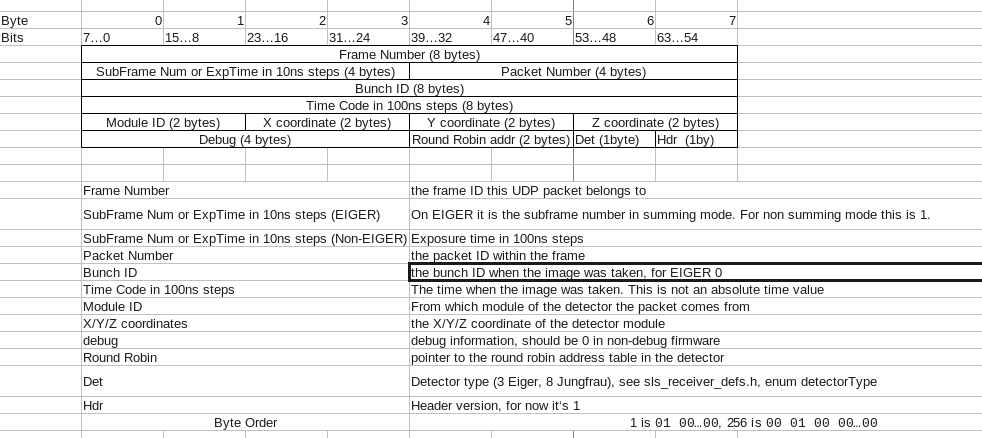
\includegraphics[width=1.2\textwidth]{EIGERUDPHeader}
\end{center}
\caption{UDP header out of EIGER}
\label{UDPheader}
\end{figure}
 
\subsection{Data out of the slsReceiver}


For a module, the geometry of the ports are as in table~\ref{tports}: 
\begin{table}
\begin{tabular}{|c|c|}
\hline
{\tt{0:rx\_udpport 50011}} &  {\tt{0:rx\_udpport2 50012}}\\  
\hline
{\tt{1:rx\_udpport 50013}} &  {\tt{1:rx\_udpport2 50014}}\\  
\hline
\end{tabular}
\caption{UDP port geometry for a single module, 4 UDP ports.}
\label{tports}
\end{table}
white the option {\tt{n:flippeddatax 1}}, which flips in vertical the content of the module. By convection, we usually use {\tt{1:flippeddatax 1}}, but one could flip the top instead.


\subsection{``raw'' files}
If you use the option of writing raw files, you will have a raw file for each UDP port (meaning most likely 2 chips), 4 files per module. In addition to the raw files, you will get also a ``master'' file, containing in ascii some detector general parameters and the explanation of how to interpret the data from the raw files.
   
The master file is named: {\tt{filename\_master\_0.raw}} and for version ``4.0.0'' of the slsDetectorSoftware looks like:
 
\begin{verbatim}
Version                    : 2.0
Dynamic Range              : 32
Ten Giga                   : 1
Image Size                 : 524288 bytes
x                          : 512 pixels
y                          : 256 pixels
Max. Frames Per File       : 10000
Total Frames               : 1
Exptime (ns)               : 1000000000
SubExptime (ns)            : 2621440
SubPeriod(ns)              : 2621440
Period (ns)                : 1000000000
Timestamp                  : Mon Sep  3 09:07:05 2018


#Frame Header
Frame Number               : 8 bytes
SubFrame Number/ExpLength  : 4 bytes
Packet Number              : 4 bytes
Bunch ID                   : 8 bytes
Timestamp                  : 8 bytes
Module Id                  : 2 bytes
X Coordinate               : 2 bytes
Y Coordinate               : 2 bytes
Z Coordinate               : 2 bytes
Debug                      : 4 bytes
Round Robin Number         : 2 bytes
Detector Type              : 1 byte
Header Version             : 1 byte
Packets Caught Mask        : 64 bytes
\end{verbatim}

Note that if one wants to  reconstruct the real time the detector was acquiring in 32 bit (autosumming mode), one would have to multiply the SubExptime (ns) for the SubFrame Number. 

\subsection{Offline image reconstruction}
The offline image reconstruction{\tt{slsImageReconstruction}} is not part of the package anymore. The code is still available doing \\
{\tt{git clone git@git.psi.ch:sls\_detectors\_software/sls\_image\_reconstruction.git slsImageReconstruction}}.
Checkout the {\tt{developer}} branch if in a 3.1.X release or the {\tt{v4.0.0}} branch if in 4.0.X release of the {\tt{slsDetector}} code.

Three possible conversions are possible: into \textbf{cbf}, \textbf{hdf5} and \textbf{root} format. The detector writes 4 raw files per receiver. An offline image reconstruction executable has been written to collate the possible files together and produce output files. By default an interpolation between the values of the large pixels is performed. Gap pixels between modules are also inserted.

Note that the number of images per file is hardcoded and needs to match whatever you are using in {\tt{slsDetectorsPackage/slsReceiverSoftware/include/sls\_receiver\_defs.h}}:
\begin{verbatim}
#define EIGER_MAX_FRAMES_PER_FILE	2000
\end{verbatim}
The default is 2000.

\subsubsection{cbf}
The cbf executable executable uses the CBFlib-0.9.5 library (downloaded from the web as it downloads architecture dependent packages at installation).Edit the Makefile to correclty point at it.\\
\underline{At cSAXS, the CBFlib-0.9.5 has been compiled -such that the required packages are}\\\underline{ downloaded in /sls/X12SA/data/x12saop/EigerPackage/CBFlib-0.9.5.}\\ 

To use it for a single module:
\begin{verbatim}
cbfMaker [filename with dir]
\end{verbatim}
eg.
{\tt{cbfMaker /scratch/run\_63\_d1\_f000000000000\_3.raw}}\\

To use it any geometry:\\
{\tt{cbfMaker [filename] [outdir, def=same as filename] [pixels x, def=1024] [pixels y, def=512] [singlemodulelongside\_x, def=1] [fillgaps, def=Interpolate Big Pixels] [hdf5datasetname, def="Eiger"] [start det,def=0]}}\\
eg.
{\tt cbfMaker /scratch/run\_63\_d0\_f000000000000\_3.raw  3072 512 1 2 ``Eiger'' 0}.\\

The {\tt{[singlemodulelongside\_x]}} {\tt{[option to interpolate gap pixels]}} param are optional. Defaults are ``1'', the detector long side is on the x coordinate and to start to reconstruct from module 0.
The interpolation scheme fro the gap pixels between chips is by default ``interpolate large big pixels'', =2;
If you want to change interpolation scheme, use:\\
\begin{tabular}{|c|c|}
\hline
interpolation scheme & argument\\
\hline
insert gap pixels and assign value only to the first one  & 0\\
\hline
equally divide the value of the counter bettern the two pixels & 1\\
\hline
interpolate large pixel value & 2\\
\hline
mask the value of the two gap pixels & 3\\
\hline
\end{tabular}
\ \\
\ \\ 
The executables: 
\begin{verbatim}
cbfMaker1.5M [file_name_with_dir]
cbfMakerOMNY [file_name_with_dir]
cbfMaker9M [file_name_with_dir]
\end{verbatim}
contain the hardcoded geometry for the 1.5M (3 modules horizontal on the long side), the 1.5M OMNY geometry (3 modules next to each other on the long side) and for the 9M at cSAXS: 6(short side)$\times$3 (long side) modules.\\ 
Missing packets in a frame and border pixels ($\times 2$ and $\times 4$ are given with value $-1$ at the present time.

Make sure the following options are uncommented in the {\tt{slsImageReconstruction/src/main\_csaxs.cpp}} file. 
\begin{verbatim}
#define MYCBF
##following line only if you need to process with 
##BUBBLE (Material Science / uXAS beamlines).
#define MSHeader 
\end{verbatim}
Compile it with: 
\begin{verbatim}
make cbfMaker; make cbfMakerOMNY;
\end{verbatim}

\subsubsection{hdf5}
In case of HDF5 output file, we rely on having the HDF5 1.10.1 library installed and {\tt{HDF5-External-Filter-Plugins}} installed. With HDF5 1.10.3, no need of the external plugings package is needed, but a small modification to the file is needed. Edit the Makefile to correclty point at it. Different compression methods are being tried so different external filters might be to be installed. This work is not finished yet.

To choose HDF5, with ZLIB implementation, open {\tt{slsImageReconstruction/src/main\_csaxs.cpp}} and make sure that 
\begin{verbatim}
#define HDF5f
#define ZLIB
\end{verbatim}
are not commented out. All other options need to be commented out. Copile the code with 
\begin{verbatim}
make hdf5Maker; make hdf5MakerOMNY;
\end{verbatim}

If you are at cSAXS. all images collected will be written in a single file. If you are not at CSAXS, most likely you want to have all the images written in a single raw file into an HDF5 file. The multiple HDF5 files are then linked in a master file, with many subdatasets (can be read by albula) or by a virtual file with a single dataset. If you want a master o virtual file, uncomment this option:
\begin{verbatim}
#define MASTERVIRTUAL
\end{verbatim}
and recompile.
To use it for a single module:
\begin{verbatim}
hdf5Maker [filename with dir]
\end{verbatim}
eg.
{\tt{hdf5Maker /scratch/run\_63\_d1\_f000000000000\_3.raw}}\\

To use it any geometry:\\
{\tt{hdf5Maker [filename] [pixels x, def=1024] [pixels y, def=512] [singlemodulelongside\_x, def=1] [fillgaps, def=Interpolate Big Pixels] [hdf5datasetname, def="Eiger"] [start det,def=0]}}\\
eg.
{\tt hdf5Maker /scratch/run\_63\_d0\_f000000000000\_3.raw  3072 512 1 2 ``Eiger'' 0}.\\

\subsubsection{root}
The data will be written as TH2D in root format. Edit the {\tt{Makefile}} to point to the correct ROOT library location. Compile the executable as:
\begin{verbatim}
make image 
\end{verbatim}
There is no program other executable that already keeps into account the geometry for it.
To use it any geometry:\\
{\tt{image [filename] [pixels x, def=1024] [pixels y, def=512] [singlemodulelongside\_x, def=1] [fillgaps, def=Interpolate Big Pixels] [hdf5datasetname, def="Eiger"] [start det,def=0]}}\\
eg.
{\tt image /scratch/run\_63\_d0\_f000000000000\_3.raw  3072 512 1 2 ``Eiger'' 0}.\\

\subsection{Read temperatures/HV from boards}

With an updated kernel on the linux boards (ask to the SLS detector group for specifications), it is possible to monitor the temperature on the boards: 
\begin{verbatim}
temp_fpga   #gets the temperature of the fpga
temp_fpgaext   #gets the temperature close to the fpga
temp_10ge   #gets the temperature close to the 10GE
temp_dcdc   #gets the temperature close to the dc dc converter
temp_sodl   #gets the temperature close to the left so-dimm memory
temp_sodr   #gets the temperature close to the right so-dimm memory
temp_fpgafl   #gets the temperature of the left front end board fpga
temp_fpgafr   #gets the temperature of the right front end board fpga

\end{verbatim}

You need to use the command specifying from which board you desire the temperature readings, for example:
\begin{verbatim}
./sls_detector_get 0:temp_fpga
./sls_detector_get 1:temp_fpga
\end{verbatim}
In 500k--2M pixel systems there is a hardware temperature safety switch, which will cut power to the BEBs when reaching a too high temperature. For the 9M system, there is a temperature sensor read by the bchip100 PCU which will shutdown the detector when above a certain temperature.
 
The HV can also be set and read through the software:
\begin{verbatim}
./sls_detector_put vhighvoltage 150
./sls_detector_get vhighvoltage 
\end{verbatim}
Note that the get {\tt{vhighvoltage}} would return the measured HV from the master module only. If getting the vhighvoltage for individual halfmodules, only the master will have a value different from -999.

\appendix

\section{Kill the server, copy a new server, start the server}\label{server}
All the below operations are form a terminal and assume you login to the boards.\\
Kill current server:
\begin{verbatim}
ssh root@bebxxx #password is root
killall eigerDetectorServer # kill server and stopserver
\end{verbatim}
Copy a new version of the server (if necessary, otherwise skip it):
\begin{verbatim}
cd executables
scp user@pc:/path/eigerDetectorServerNewVersion .
chmod 777 eigerDetectorServerNewVersion
mv eigerDetectorServerNewVersion eigerDetectorServer
sync
\end{verbatim}
Start the server again:
\begin{verbatim}
./eigerDetectorServer &
\end{verbatim}
\textbf{Note that the server appropriate for the software version used is located inside the package: {\tt{slsDetectorsPackage/serverBin/eigerDetectorServerxx.yy.}}}.

To copy the detector server on many boards, a script can be implemented on the lines of:
\begin{verbatim}
for i in beb111 beb070; 
do ssh root@$i killall eigerDetectorServer; 
scp eigerDetectorServer root@$i:~/executables/eigerDetectorServer ; 
ssh root@$i sync; done
\end{verbatim}

\section{Loading firmware bitfiles}

\textbf{As a new procedure, the first thing to do is to kill the server on the boards, copy the new one there without starting it.} Note that failure to do this step before may cause the linux on the boards to crash and not being able to ping it (this if the registers between the old and new firmware change).

This is the procedure from a terminal;
\begin{verbatim}
for i in beb111 beb070; 
do ssh root@$i killall eigerDetectorServer; 
scp eigerDetectorServer root@$i:~/executables/eigerDetectorServer ; 
ssh root@$i sync; done
\end{verbatim}

A \textbf{bcp} executable (which needs \textbf{tftp} installed on the PC, is needed. 
\begin{enumerate}
\item Manual way: you need to press something on the detector. To program bitfiles (firmware files), do a hard reset with a pin/thin stuff in the holes at the very back of the module. They are between the top 7 LED and the bottom 1 and opposite for the other side. Push hard till all LEDs are alternating green and red.
\item Software way (possible only if you have the correct programs copied on your board. If not, as the sls detector group). 
\begin{verbatim}
ssh root@bebxxx
cd executables
./boot_recovery 
 \end{verbatim} 
\end{enumerate}
In both case, after booting, only the central LED should be on green and red alternating. 

From a terminal, do:
\begin{verbatim}
nc -p 3000 -u bebxxx 3000 
\end{verbatim} 
where {\tt{xxx}} is the board number. It is enough top monitor with {\tt{nc}} only one board. Pres enter twice (till you see a prompt with the board hostname printed) and keep this terminal to monitor. It takes a bit of time to load the bitfiles, but the terminal tells you.\\
From another terminal you do:
\begin{verbatim}
./bcp feb_left.bit bebxxx:/febl
sleep 300; #or till the screen over netcat has told you Successful
./bcp feb_right.bit bebxxx:/febr
sleep 300; #or till the screen over netcat has told you Successful
./bcp download.bit bebxxx:/fw0
sleep 300; #or till the screen over netcat has told you Successful
\end{verbatim}
If you need to program a new kernel (only needed when told to do so):
\begin{verbatim}
 ./bcp kernel_local bebxxx:/kernel
sleep 300; #or till the screen over netcat has told you Successful
\end{verbatim}
do the same for the other boards. You can program in parallel many boards, but you cannot load two bitfiles on the same board till loading and copying one process has finished. So load all left febs together, then proceed to the right febs, then the bebs. Power off completely everything. Power it on.

\section{Pulsing the detector}
There are two ways to pulse the detector: 
\begin{itemize}
\item \textbf{Pulse digitally:} when you are interested to the output readout and do not care about the analog response from the pixels:
 \begin{verbatim}
sls_detector_put vthreshold 4000
sls_detector_put vtr 4000
sls_detector_put pulsechip N #to pulse N
sls_detector_put pulsechip -1 #to get out of testing mode 
\end{verbatim}
Note that the answer will be $2 \cdot \textrm{{\tt{N}}} +2$ in this case.

\item  \textbf{Pulse analogically:} You want to really check the analogical part of the detector, not just the readout.

 \begin{verbatim}
sls_detector_put vcall 3600
sls_detector_put vthreshold 1700
sls_detector_put vrf 3100
for i in $(seq 0 7) ; 
do px=$((-255+i)); 
sls_detector_put  pulse 0 $px 0;
for j in $(seq 0 255) ; do
sls_detector_put pulsenmove N 0 1;
done;
done;
sls_detector_put resmat 0
sls_detector_acquire
\end{verbatim}
You read {\tt{N}} in every pixel if you are setup correctly. 
\end{itemize}
 
\section{Load a noise pattern with shape}
For debug purposes, we have created a noise pattern with a shape. If you reconstruct correctly your image, you should be able to read ".EIGER'' in the same direction for both the top and bottom in normal human readable orientation.
To load the special noise file look at {\tt{settingsdir/eiger/standard/eigernoise.sn0xx}} in the package. 
\begin{verbatim}
sls_detector_put trimbits ../settingsdir/eiger/standard/eigernoise
\end{verbatim}
To exit from this pattern noise, just set the threshold to something known. 
\begin{verbatim}
\item sls_detector_put threshold 50000 standard
\end{verbatim}
where 5000 would be a value in eV and {/tt{standard}} is important in this case.

\section{(Fast) threshold scans during beam operation}\label{sec:fastthresholdscan}
Occasionally you might need to do threshold scans during your data taking (for example for Laue experiments or to get any spectral information). Setting the threshold in this case would be not optimal as you would change trimbits at every energy and this could give you a ``step'' behaviour. What you could do is to use the 
\begin{verbatim}
\item sls_detector_put thresholdnotb 50000 
\end{verbatim}
 which set the threshold to an energy but does not change trimbits. We suggest that before using this function you load the {\tt{threshold}} at an energy in the middle of your scan range and then change {\tt{thresholdnotb}}.
We have also been requested if we could speed up the threshold scan. At the moment no specific function has been integrated in firmware, but one could use the software trigger option to perform what you need:
\begin{verbatim}
./sls_detector_put exptime 0.01
./sls_detector_put timing trigger
./sls_detector_put enablefwrite 0
./sls_detector_put resetframescaught 0 
./sls_detector_put index 0
./sls_detector_put cycles 21
./sls_detector_put receiver start
./sls_detector_put status start 
for i in $(seq 0 20); 
 do
   #./sls_detector_put thresholdnotb 5000 ##this is still too slow as it loads the module 
 ./sls_detector_put 0:vrf 3199 #need to know the appropriate vrf at every energy 
 ./sls_detector_put 1:vrf 3199 #need to know the appropriate vrf at every energy 
 ./sls_detector_put status trigger
    #sleep 0.005
done
./sls_detector_put  receiver stop
./sls_detector_put  resetframescaught 0 
./sls_detector_put  timing auto
\end{verbatim} 

\section{Troubleshooting}
\subsection{Cannot successfully finish an acquisition}
\subsubsection{Only master module return from acquisition}
When no packets are received AND detector states in 'running status'. Widest list of causes. 
Query the status of each half module till the maximum number {\tt{N}},  {\tt{for i in \$(seq\ 0\ N); do sls\_detector\_get \$i:status; done}}, to check if there are half modules that are still running.

If only the master modules return but ALL the other half modules do not: 
\begin{itemize}
\item FEB LED 1 and or 3 become red while trying to acquire an image: reconnect or change the DDR2 memories. Technically it is a FIFO problem to communicate the data to the rest of the chain. 
\item It can be that the master cable is not connected, check.
\item It can be that the synchronization cable is not connected or the termination board at the synchronization does not work. Check.
\end{itemize}

\subsubsection{A few modules do not return from acquisition}
If only a few modules are still running but the others return, it is a real problem with a backend board or a synchronization bug.
If you can, ssh into the board, kill and start the eigerDetectorServer again (see Section~\ref{server} for how to do this). Keep the terminal with the output from the  eigerDetectorServer and repeat the acquisition. 
\begin{itemize}
\item Check if the acquisition returned from the server or not. In case seek help from the SLSDetectorGroup.
\item In the server you read something along the lines of "cannot read top right address". It is communication between the front and backend board. Or FEB FPGA is not programmed. Try to program again FPGA, and make sure you program FPGA bit files 70x, if you have 70x FPGAs, or 30x, if you have 30x FPGAs. If still fails, tell the SLSDetectorGroup as it could be a hardware permanent failure.
\end{itemize}

\subsection{No packets (or very little) are received} 
In both cases running \textbf{wireshark} set to receive UDP packets on the ethernet interface of the receiver (filter the UDPport$>=$xxxx, where xxxx is written in the configuration file) can help you understanding if NO packets are seen or some packets are seen. You have to set the buffer size of the receiving device in wireshark to 100Mbyte minimum. If no packets are received, check that your receiving interface and detector UDPIPs are correct (if in 10Gb). Most of the time in this case it is a basic configuration problem.
It can help looking at the receiver output, shown in an example here:
\begin{verbatim}
Missing Packets         : 224064
Complete Frames         : 3499
Last Frame Caught       : 3499
\end{verbatim}

The {\tt{Last Frame Caught}}, meaning the packet from the last frame that was sent out by the detector, can help in understanding the problem: 
\begin{enumerate}
\item If some packets are received, but not all, it could be a network optimization problem. In this case, the {\tt{Last Frame Caught}} will be a value close to the expected number of frames with missing frames distributed over the whole frame range. In this case: 
 \begin{itemize}
\item For receiving data over 1Gb, the switch must have FLOW CONTROL enabled 
\item If using 10GbE, check that the 10Gb link is active on the backpanel board. Then refer to Section~\ref{10g} to see how to configure the 10Gb ports on the receiving machine correctly. 
\end{itemize}
\item If the {\tt{Last Frame Caught}} value is much lower than the expected frames and you are missing a bunch of frames from a point onwards, and you are using {\tt{receiver start, status start}}: then it can be that you are stopping the receiver too early. In particular when you are using {\tt{delay}} it might be that there is some time between when the detector is already done and in {\tt{idle}} state but the receiver is still receiving data. Check with {\tt{./sls\_detector\_get framescaught}} if the receiver is already done before doing {\tt{./sls\_detector\_put receiver stop}}.   
\item If the {\tt{Last Frame Caught}} value is much lower than the expected frames and you are missing a bunch of frames from a point onwards and you are running at a higher frame rate than the continuous framerate (see table~\ref{tcont}) with more images than the size of the memory (see table~\ref{timgs}). It might be that you are running out of memory to store images. There is no protection for this. see point~\ref{outmemory}
 \end{enumerate}

\subsection{'Got Frame Number Zero from Firmware'}\label{outmemory}
In this case, you have run out of memory size (see table~\ref{timgs} for the size) on the boards so you are trying to store on the DDR2 memories more images that they can contain and the network is not fast enough to send everything out from the 10GbE.
So if you see:
\begin{verbatim}
Got Frame Number Zero from Firmware. Discarding Packet
\end{verbatim}
it means that you run out of memory at the previous acquisition. The  cure is taking 2 or 3 SINGLE images in a raw to clear out the memories.
 


\subsection{The module seems dead, no lights on BEBs, no IP addresses}
\begin{itemize}
\item Check the 2 fuses on the power distribution board. If one of the fuses is in shortcuircuit, then exchange it. Nominal values are 7 A and 5 A. Old modules with 5 A and 3 A could trip.
\item The module is not properly cooled and the temperature safety switch has killed the power to the backend boards. 
\end{itemize}

\subsection{The module seems powered but no IP addresses}
If the 1G LED (see Section~\ref{led}) on the backpanel board is not green:
\begin{itemize}
\item Check that the 1Gb cable is plugged in.
\item Check that there is a DCHP server assigning IP addresses to the board.
\item The IP address is assigned only at booting up of the boards. Try to reboot in case the board booted before it could have an IP address. 
\item Check that you did not run out of IP addresses 
\end{itemize}
 Check that the board is not in recovery mode (i.e. the central LED on the back is stable green, see Fig~\ref{fLEDs}). In this case reboot the board with the soft reset or power cycle it.

If the 1Gb LED on the backpanel board is green (see Section~\ref{led}):
\begin{itemize}
\item Check that the IP address has been refreshed on the PC you are trying to communicate to the detector from. Run on the PC as root the following command to update the DNS cache: \textbf{nscd -i hosts} 
\end{itemize}

\subsection{Receiver cannot open socket}
It is connected to the TCPport which the receiver uses:
\begin{itemize}
\item The port is already in use by the same receiver already opened somewhere or by another process: check with \textbf{ps -uxc} your processes
\item In rare cases, it might be that the TCP port crashes. To find out which process uses the TCPPOrt do: \textbf{netstat -nlp | grep xxxx}, where xxxx is the tcpport number. To display open ports and established TCP connections, enter: \textbf{netstat -vatn}. Kill the process.
%%%#To display only open UDP ports try the following command: netstat -vaun
 \end{itemize}

\subsection{The client ignores the commands}
Make sure that in the configuration file you do not have {\tt{lock 1}} activated, as this will let only one username from one IP address talk to the detector. 
To deactivate it, you need to run {\tt{lock 0}} from the client session where you locked it. 

\subsection{Zmq socket is blocked}
It is connected to the TCPport which is used. In rare cases, it might be that the TCP port crashes. To find out which process uses the TCPPOrt do: \textbf{netstat -nlp | grep xxxx}, where xxxx is the tcpport number. To display open ports and established TCP connections, enter: \textbf{netstat -vatn}. Kill the process.


\subsection{Client has \textbf{shmget error}}
Note that occasionally if there is a shared memory of a different size (from an older software version), it will return also a line like this:
\begin{verbatim}
*** shmget error (server) ***-1
\end{verbatim}
This needs to be cleaned with {\tt{ipcs -m}} and then {\tt{ipcrm -M xxx}}, where xxx are the keys with nattch 0. Alternative in the main slsDetectorFolder there is a script that can be used as {\tt{sh cleansharedmemory.sh}}. Note that you need to run the script with the account of the client user, as the shared memory belongs to the client. It is good procedure to implement an automatic cleanup of the shared memory if the client user changes often.   

\subsection{Client has shared memory iusses}
The shared memory from software version 4.0.0 creates shared memory segments in /dev/shm/. You can look at them and cancel them directly. Note that this is still user dependent.
Environment variable SLSDETNAME can be set for using 2 different detectors from the same client pc. One needs a different multi detector id if the SLSDETNAME is different for both consoles.

\subsection{Measure the HV}
For every system: 
\begin{itemize}
\item Software-wise measure it (now the software returns the measured value), with {\tt{sls\_detector\_get vhighvoltage}}. The returned value is the HV (for proper Eiger setting is approximately 150~V) if it is correctly set. If two master modules are presents (multi systems), the average is returned (still to be tested). If one asks for the individual $n$ half module bias voltage through {\tt{sls\_detector\_get n:vhighvoltage}}, if the $n$ module is a master, the actual voltage will be returned. If it is a slave, -999 will be returned. 
\item Hardware-wise (opening the detector) measure value of HV on C14 on the power distribution board. Check also that the small HV connector cable is really connected. 
 \end{itemize}

The 2M system at ESRF has a HV enable signal that needs to be shortcut in order to overwrite vacuum protections (when not in vacuum). 
The 1.5M for OMNY has a relay system that enables HV only when the vacuum is good. 
For both systems, it makes sense not to set the HV while running the configuration file but set it at a later stage when sure about the vacuum. 

\subsection{The image now has a vertical line}
Check if the vertical line has a length of 256 pixels and a width of 8 columns. In this case it is a dataline being bad. It can be either a wirebond problem or a frontend board problem. try to read the FEB temperature (see Section~\ref{}) and report the problem to the SLSDetector group. Most likely it will be a long term fix by checking the hardware.

\subsection{The image now has more vertical lines}

If you see strange lines in vertical occurring at period patterns, it is a memory problem. The pattern is 4 columns periodic in 16 bit mode, 8 columns periodic in 8 bit mode and 2 columns periodic in 32 bit mode. Try to switch on and off (sometimes it is a strange initialization problem).

\subsection{ssh to the boards takes long}
Depending on your network setup,  to speed up the ssh to the boards from a pc with internal dhcp server running: \textbf{iptables -t nat -A POSTROUTING -o eth1 -j MASQUERADE; echo "1" > /proc/sys/net/ipv4/ip\_forward}, where eth1 has to be the 1Gb network device on the pc

\subsection{Generate keys on the boards not to have to type the password}
\begin{verbatim}
export AFSDIRS64=/afs/psi.ch/intranet/Controls/Software/Trolltech/SL6-x86_64
ssh-copy-id -i /afs/psi.ch/user/t/tinti_g/.ssh/id_rsa.pub  root@beb100
ssh-keygen
\end{verbatim}

\subsection{Check firmware version installed on BEB}
You can either ask in the client as described in section~\ref{api}, or login to the boards directly. Follow some steps described in Section~\ref{server}. 
\begin{verbatim}
ssh root@bebxxx #password is root
killall eigerDetectorServer # kill server and stopserver
cd executables/
./eigerDetectorServer&
\end{verbatim}
Scroll up in the terminal till you find {\tt{Firmware Version: xx}}

\subsection{Check if half-module is a master, a slave, a top or a bottom}
Follow some steps described in Section~\ref{server}.
\begin{verbatim}
ssh root@bebxxx #password is root
killall eigerDetectorServer # kill server and stopserver
cd executables/
./eigerDetectorServer&
\end{verbatim}
Scroll up in the terminal till you find:\\
*************** TOP/BOTTOM ***************\\
*************** MASTER/SLAVE ***************\\
*************** NORMAL/SPECIAL ***************\\

There is also an easier way, that is that only the master module will return the real value of the HV. If you have more than 1 detector system, then you will have more than 1 physical master, as the HV needs to be applied to all the systems.

\begin{verbatim}
for i in $(seq 0 36); do sls_detector_put $i:vhighvoltage; done
\end{verbatim}
 Only the master will return to you a sensible number (150 normally). the others will return -999.

\subsection{'Cannot connect to socket'}
This error is typically due to the detector server not running. For why, see section~\ref{servernot}.

\subsection{Running at low frame rate, the communication to receiver stops}
If running in 32-bit mode (or even in 16-bit mode), if more memory than what your machine can handle is asked for, the receiver process could be terminated by the kernel of your machine. It would loook like you had executed a clean control-c on the receiver executable. This has been the case, when setting up by mistake
\tt{rx\_fifodepth} to 10000 images in 32 bit mode. In 32 bit mode it will assign 40~GB of memory, which is more than what normal PC would have. So make sure you do not require too much memory. The same is tru also for smaller values of {\tt{rx\_fifodepth}} if your  machine has not much memory.  

\subsection{Detector server is not running}\label{servernot}
The detector server could not be running: either the detector was powered off, or it powered off itself due to too high temperature or, in the case of the 9M, if the waterflow sensor detected no flux and powered it off (the chiller stops occasionally as cSAXS).

If the powering and the temperature are OK, instead, it can be that the firmware version is incompatible to the server version and/or the client software version. In software packages 3.x.y, the eigerDetectorServer was killed automatically. So check the consistency of firmware/software/server versions if using this version of the software. From 4.x.y onwards, the server, if associated to a wrong firmware, does not kill itself.   

\subsection{'Acquire has already started' error message}
If you see the client returning the following error message:\\ 
``Acquire has already started. If previous acquisition terminated unexpectedly, reset busy flag to restart.(sls\_detector\_put busy 0)''\\
 You need to run the command:
\begin{verbatim}
./sls_detector_put busy 0
\end{verbatim}

\subsection{There is noise running the detector in 32-bit}
If you are running the detector in 32-bit (autosumming), there might be some noise, particularly at lower threshold energies. This is due to the fact that the analog part of the chips require some latency time to settle which is larger than the readout time. It is possible to run the detector only in {\tt{parallel}} or {\tt{nonparallel}} mode, respectively with readout times between frames of 12~$\mu$s and 504~$\mu$s. If you switch {\tt{flags}} to non {\tt{nonparallel}} mode you will give enough time for the signals to settle. From release 4.0.0, there is a configurable delay that can be set through the {\tt{subdeadtime}} variable, such that you can remain with the {\tt{parallel}} flag, but can obtain a configurable dead time between frames. Ask the SLS detector group for an appropriate dead time for your detector, but typically a dead time of 20-50~$\mu$s should be enough. Note that this {\tt{subdeadtime}} need to include the 12~$\mu$s minimum readout time, so it has to be larger than 12~$\mu$s to do anything.  
 
\subsection{There is noise running the detector at high frame rate(4,8,16 bit)}
If are running in {\tt{parallel}} mode, in particular at low threshold energies, you might encounter some noise. The reason is that the analog part of the chips require some latency time to settle which is larger than the readout time. 
\begin{enumerate}
\item You can lower the frame rate and relax requirements on period: 
At low frame rate, you normally leave enough time between the end of the acquisition and the starting of the next, so you should not see this effect. In any case setting a {\tt{period}}={\tt{exptime}}+readout time from Table~\ref{tchipro} +extra 20$\mu$s cures the problem. The 20$\mu$s could also be 10~$\mu$s, they are very hardware dependent.
\item The frame rate requirement are stringent (as for time resolved measurements): the only option here is to reduce the {\tt{exptime}} to let the extra 20~$\mu$s (or 10)~$\mu$s. The {\tt{period}} remains the same.
\end{enumerate} 
 
\section{Client checks - command line}

Guide on returned strings:
\begin{enumerate}
\item \begin{verbatim}
sls_detector_get free
\end{verbatim}
Returns a list of shared memories cleaned (variable number depending on detector):
\begin{verbatim}
Shared memory 273612805 deleted
Shared memory 276922374 deleted
Shared memory 270270468 deleted
free freed
\end{verbatim}
Note that occasionally if there is a shared memory of a different size (from an older software version), it will return also a line like this:
\begin{verbatim}
*** shmget error (server) ***-1
\end{verbatim}
This needs to be cleaned with {\tt{ipcs -m}} and then {\tt{ipcrm -M xxx}}, where xxx are the keys with nattch 0. 
\item \begin{verbatim}sls_detector_get settings
settings standard
\end{verbatim} 
{\tt{standard}} is only if correct. {\tt{undefined}} or anything else is wrong. 

\item \begin{verbatim}
sls_detector_get threshold
threshold xxxx
\end{verbatim}
Returns a string (xxxx) that can be interpreted as the threshold in eV. If it fails to set it, returns the last threshold it was set (which the detector still has). If settings are not defined or different trimbits are chosen, it will return "undefined".

\item \begin{verbatim}
sls_detector_get fname
fname string
\end{verbatim}

\item \begin{verbatim}
sls_detector_get exptime
exptime number
\end{verbatim}
where {\tt{number}} is a string to be interpreted as a float in (s). 

\item \begin{verbatim}
sls_detector_get period
period number
\end{verbatim}
where {\tt{nuymber}} is a string to be interpreted as a float in (s). 

\item \begin{verbatim}
sls_detector_get frames
frames number 
\end{verbatim}
where {\tt{number}} is a string to be interpreted as an integer.

\item \begin{verbatim}
sls_detector_get cycles
cycles number 
\end{verbatim}
where {\tt{number}} is a string to be interpreted as an integer.

\item \begin{verbatim}
sls_detector_get status
status string 
\end{verbatim}
where {\tt{string}} can be {\tt{idle}} or {\tt{running}}.

\item \begin{verbatim}
sls_detector_get index
status number
\end{verbatim}
where {\tt{number}} is a string to be interpreted as an integer.

\item \begin{verbatim}
sls_detector_get dr
dr number
\end{verbatim}
where {\tt{number}} is a string that should be interpreted as an integer (4/8/16/32).

\item \begin{verbatim}
sls_detector_get clkdivider
clkdivider number
\end{verbatim}
where {\tt{number}} is a string that should be interpreted as an integer (0/1/2/3).

\item \begin{verbatim}
sls_detector_get flags
flags string1 string2 
\end{verbatim}
where {\tt{string1}} is a string should be always {\tt{continous}} and {\tt{string2}} can be either {\tt{nonparallel}} or {\tt{parallel}}.

\item \begin{verbatim}
sls_detector_get timing 
timing string
\end{verbatim}
where {\tt{string}} is a string which can be {\tt{auto/trigger/burst\_trigger/gating}}.

\item \begin{verbatim}
sls_detector_get enablefwrite
enablefwrite number
\end{verbatim}
where {\tt{number}} is a string which should be interpreted as an integer "0" or "1".

\item \begin{verbatim}
sls_detector_get framescaught
framescaught number
\end{verbatim}
where {\tt{number}} is a string which should be interpreted as an integer of the complete frames got by the receiver.

\item \begin{verbatim}
sls_detector_get frameindex
frameindex number
\end{verbatim}
where {\tt{number}} is a string which should be interpreted as an integer of the last frame number read from firmware. It comes from the receiver, though and reset after every acquisition series.

\item \begin{verbatim}
sls_detector_get subexptime
subexptime number
\end{verbatim}
where {\tt{number}} is a string that should be interpreted as a float in s. The default value is 0.002621440. 

\item \begin{verbatim}
sls_detector_get ratecorr
ratecorr number
\end{verbatim}
where {\tt{number}} is a string that should be interpreted as a float in s.  0.000000 means correction off. Values above zero are the value of $\tau$ in ns.

\item \begin{verbatim}
sls_detector_get vhighvoltage
vhighvoltage number
\end{verbatim}
where {\tt{number}} is a string that should be interpreted as an int and for proper Eiger setting is approximately 150~V if it is correctly set. If two master modules are presents (multi systems), the average is returned (still to be tested). If one asks for the individual $n$ half module bias voltage through {\tt{sls\_detector\_get n:vhighvoltage}}, if the $n$ module is a master, the actual voltage will be returned. If it is a slave, -999 will be returned. 
  
\item \begin{verbatim}
sls_detector_get busy
busy number
\end{verbatim}
where  {\tt{number}} is a string that should be interpreted as an int for 0/1 meaning no/yes. This command tells if the sharedmemory has in memory that an acquisition has been started or not. It should allows to use the non blocking acquire, regardless of any delay to the detector getting into 'running' mode. 


\end{enumerate}

\section{Complete data out rate tables}

In table~\ref{tframescomplete} is a list of all the readout times in the different configurations.
\begin{tiny}
\begin{table}
\begin{flushleft}
\begin{tabular}{|c|c|c|c|c|c|c|}
\hline
\tiny{dr} & \tiny{clkdivider} & \tiny{flags} & \tiny{readout t($\mu$s)} & \tiny{max frame rate (kHz)} & \tiny{min period ($\mu$s)} & \tiny{max imgs (nominal/our network)}\\
\hline
4 & 0 & parallel & 3.4 & 22 &  44 & 30k/50k\\
\hline
4 & 0 & nonparallel & 44 & 21 & 49 & 30k/50k\\
\hline
4 & 1 & parallel & 6 & 10.5 &  92 & 30k/100k\\
\hline
4 & 1 & nonparallel & 88.7 & 10.5 & 93 & 30k/100k\\
\hline
4 & 2 & parallel & 11.2 & 5.4 & 197 & infinite\\
\hline
4 & 2 & nonparallel & 176.5 & 5.4 & 180 & infinite\\
\hline
\hline
8 & 0 & parallel & 3.4 & 11.1 & 89 & 15k/24k\\
\hline
8 & 0 & nonparallel & 85.7 & 11.1 & 91 & 15k/24k\\
\hline
8 & 1 & parallel & 6.1 & 5.7 & 181 & 15k/52k\\
\hline
8 & 1 & nonparallel & 170.5 & 5.7 & 175 & 15k/52k\\
\hline
8 & 2 & parallel & 11.2 &  2.9 &  342 & infinite\\
\hline
8 & 2 & nonparallel & 340.3 &  2.9 &  344 & infinite\\
\hline
\hline
16 & 0 & parallel & 3.4 & 6.1 & 164 & 8k/12k\\
\hline
16 & 0 & nonparallel &  126 & 5.6& 179 & 8k/23k\\
\hline
16 & 1 & parallel &  6.1 & 3.9&  257 & 8k/28k\\
\hline
16 & 1 & nonparallel & 255 & 3.3&  303 & infinite\\
\hline
16 & 2 & parallel &  11 & 1.9  & 526 &infinite \\
\hline
16 & 2 & nonparallel & 504 & 1.8 & 555 & infinite\\
\hline
\hline
32 & 2 & parallel &  11 & 2  & &\\
\hline
32 & 2 & nonparallel & 504 & $<2$  & &\\
\hline
\end{tabular}
\caption{Readout settings. The {\tiny{min exptime}} possible is 5$-$10~$\mu$s. This is due to the time to pass the pixel enable signal in the whole chip.}
\label{tframescomplete}
\end{flushleft}
\end{table}
\end{tiny}

Table~\ref{tx} shows the bandwidth of data transferring between the FEB and BEB and of the DDR2 memory access. the GTX lanes are only capable of 25.6~Gbit/s. This limits the 12/16 bit frame rate. The 2$\times$DDR2 memories have a bandwidth or 2$\cdot$25.6~Gb/s=51.2~Gb/s. Due to this memory access bandwidth, the 32 bit autosumming mode can only run in {\tt{clkdivider}} 2.   
\begin{figure}[t]
\begin{center}
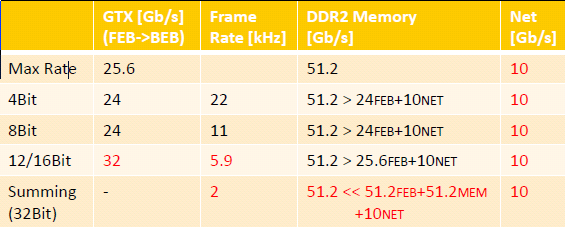
\includegraphics[width=1.\textwidth]{TansmissionRates}
\end{center}
\caption{Transmission bandwidth for the FEB $\to$BEB transfer (second column) and the DDR2 memories (fourth column). }
\label{tx}
\end{figure}

\end{document}

